\documentclass[co439]{subfiles}

%% ========================================================
%% document

\begin{document}

    \section{Geometry of Grobner Degeneration}
    
    \subsection{Integral Weight Order}

    \begin{example}{}
        Let $I = \left< xy-1 \right>\subseteq\R\left[ x,y \right]$. Then $V_{\infty}\left( I \right)$ is the hyperbola of $y=\frac{1}{x}$ whereas $V_{\infty}\left( \in\left( I \right) \right)$ consists of precisely the $x,y$-axes. We are going to investigate how this \textit{degeneration} happens in a continuous fasion.

        Consider adding a dimension to the picture and the polynomial
        \begin{equation*}
            xy-t\in\R\left[ x,y,t \right]   .
        \end{equation*}
        Then observe that the $x,y$ cross section at $t=0$ is the $x,y$-axes and the cross section at $t=1$ is the $y=\frac{1}{x}$ hyperbola.

        We call $V_{\infty}\left( xy-t \right)$ a \textit{hyperbolic paraboloid}. We can think about hyperbolic paraboloid $P$ as a \textit{family} of conics over a line. That is, there is a projection
        \begin{equation*}
            \begin{aligned}
                \phi:P&\to\R\\
                \left( x,y,t \right) & \mapsto t
            \end{aligned} 
        \end{equation*}
        and a \emph{fibre} at $t=t_0$
        \begin{equation*}
            \pi^{-1}\left( t_0 \right) = \left\lbrace \left( x,y,t \right)\in P : t=t_0 \right\rbrace,
        \end{equation*}
        so that the family $\left\lbrace \pi^{-1}\left( t \right) \right\rbrace_{t\in\R}$ completely describes $P$. Each fibre is a hyperbola, except $\pi^{-1}\left( 0 \right)$ which is the union of two orthogonal lines.

        We call this family $\left\lbrace \phi^{-1}\left( t \right) \right\rbrace^{}_{t\in\R}$ is \emph{flat} if $\pi$ is flat.
    \end{example}

    \rruleline
    
    \begin{definition}{\textbf{Isomorphic} Scheme}
        Let $I\subseteq S, J\subseteq R$ be ideals in polynomial rings $S,R$. We say $V_{\infty}\left( I \right),V_{\infty}\left( J \right)$ are \emph{isomorphic} and write $V_{\infty}\left( I \right)\iso V_{\infty}\left( J \right)$ if $S /I\iso R /J$ as rings.
    \end{definition}

    \begin{example}{}
        For over $P$, all the fibres $\pi^{-1}\left( t \right)$ for $t\neq 0$ are isomorphic. That is,
        \begin{equation*}
            \R\left[ x,y \right] / \left< xy-t_0 \right> \iso \R\left( x,x^{-1} \right) , \hspace{1cm}\forall t_0\neq 0.
        \end{equation*}
        We call each $\R\left[ x,y \right] / \left< xy-t_0 \right>$ for $t_0\neq 0$ a \textit{general fibre} and $\R\left[ x,y \right] / \left< xy \right>$ a \textit{special fibre}. Hence we have degenerated the general fibre to the special one.  
    \end{example}

    \rruleline
    
    \np In general, we chose an \emph{integral weight function}
    \begin{equation*}
        \lambda:\Z^n\to\Z,
    \end{equation*}
    which is $\Z$-linear.

    This gives a partial order $\leq_{\lambda}$, called an \emph{integral weight order}, on monomials by comparing the weights:
    \begin{equation*}
        m_1 \leq_{\lambda} m_2 \iff \lambda\left( m_1 \right)\leq\lambda\left( m_2 \right)
    \end{equation*}
    for all monomials $m_1,m_2$.

    \begin{definition}{\textbf{Initial Form} with respect to Integral Weight Order}
        Let $\leq_{\lambda}$ be an integral weight order. Given $g\in S$, we define the \emph{inital form}, denoted as, $\initial_{\lambda}\left( g \right)$, to be the sum of all the maximal terms with respect to $\leq_{\lambda}$.
    \end{definition}

    \np The next theorem shows that integral weight orders are enough to capture all initial ideals.
    
    \begin{theorem}{}
        Let $<$ be a monomial order and let $\left\lbrace g_k \right\rbrace^{n}_{k=1}$ be a Grobner basis for $I$ with respect to $<$. Then there is a finite set of pairs of monomials
        \begin{equation*}
            m_1^1 < m_2^1 , \ldots, m_1^r<m_2^r
        \end{equation*}
        such that for any integral weight order $<_{\lambda}$ with
        \begin{equation*}
            m_1^1 <_{\lambda} m_2^1 , \ldots, m_1^r<_{\lambda}m_2^r,
        \end{equation*}
        we have that
        \begin{equation*}
            \initial_{\lambda}\left( I \right) = \left\lbrace \initial_{\lambda}\left( g \right) \right\rbrace^{}_{g\in I}
        \end{equation*}
        is a monomial ideal with
        \begin{equation*}
            \initial_{\lambda}\left( I \right) = \initial_{<}\left( I \right)
        \end{equation*}
        and $\left\lbrace g_k \right\rbrace^{n}_{k=1}$ is a $<_{\lambda}$-Grobner basis for $I$ (i.e. $\initial_{\lambda}\left( I \right) = \left< \initial_{\lambda}\left( g_k \right) \right>^n_{k=1}$).
    \end{theorem}

    \begin{proof}
        For each $g_k$ and each non-initial monomial $m\in\supp\left( g_k \right)$, put
        \begin{equation*}
            m < \initial_{<}\left( g_k \right).
        \end{equation*}
        Let $\mF$ be the set of such pairs. Now imagine running Buchberger's algorithm on $\left\lbrace g_k \right\rbrace^{n}_{k=1}$, to verify that it is a Grobner basis. This yields quadratically many $S$-polynomials. Run division algorithm on each. Each time we need to identify a leading term of some polynomial $f$, add $\left( m<\initial_{<}\left( f \right) \right)$ to $\mF$ for each $m\neq\initial_<\left( f \right)$ in $\supp\left( f \right)$.

        Now take any integral weight order $<_{\lambda}$ which agrees on $\mF$. That is, for all $\left( m<f \right)\in\mF$, $m<_{\lambda}f$. If we run Buchburger's algorithm on $\left\lbrace g_1,\ldots,g_n \right\rbrace$ with respect to $<_{\lambda}$, the process is exactly the same; the division algorithm and Buchberger's criterion all work fine for partial orders provided that every initial form encountered is a single term.

        Thus $\left< \initial_{\lambda}\left( g_k \right) \right>^n_{k=1} = \initial_{\lambda}\left( I \right)$. 
    \end{proof}

    \np Here is the general idea of the degeneration. Let $k=\CC$ and let $\hat{t}\in\CC$ be nonzero. Also fix an integral weight order $\leq_{\lambda}$. Then
    \begin{equation*}
        \begin{aligned}
            \phi_{\lambda}^j: S&\to S \\
            x_j & \mapsto x_j\hat{t}^{-\lambda\left( x_j \right)}
        \end{aligned} 
    \end{equation*}
    is an automorphism of rings.

    Note that the composition of two $\phi_{\lambda}^{j_1},\phi_{\lambda}^{j_2}$ is commutative. Define
    \begin{equation*}
        \phi_{\lambda} = \phi_{\lambda}^1 \circ \cdots \circ \phi_{\lambda}^nr
    \end{equation*}
    which is also an automorphism. Since $\phi_{\lambda}$ is an automorphism, it follows that
    \begin{equation*}
        S /I \iso S /\phi_{\lambda}\left( I \right)
    \end{equation*}
    for all ideal $I\subseteq S$. But as $\hat{t}\to 0$, 
    \begin{equation*}
        \phi_{\lambda}\left( I \right) \to \initial_{\lambda}\left( I \right),
    \end{equation*}
    because the leading form starts to dominate.

    To do this better, let
    \begin{equation*}
        T = S\left[ t \right]
    \end{equation*}
    be a polynomial ring in $1$ more variable. For $f\in S$, let $\tilde{f}\in T$ be defined by
    \begin{equation*}
        \tilde{f} = t^M\phi_{\lambda}\left( f \right),
    \end{equation*}
    where $M = \max_{m\in\supp\left( f \right)} \lambda\left( m \right)$. In other words,
    \begin{equation*}
        \tilde{f} = t^Mf\left( t^{-\lambda\left( x_1 \right)}x_1, \ldots, t^{-\lambda\left( x_n \right)}x_n \right).
    \end{equation*}
    Note that the leading form $\initial_{\lambda}\left( f \right)$ remains unchanged, since we are multiplying by $t^{M}$. But all other terms have $t$. 

    For an ideal $I\subseteq S$, let
    \begin{equation*}
        \tilde{I} = \left< \tilde{g} \right>_{g\in I} \subseteq S\left[ t \right]. 
    \end{equation*}
    Then $V_{\infty}\left( \tilde{I} \right)$ is a \emph{flat family} with general fibre isomorphic to $V_{\infty}\left( I \right)$ and special fibre isomorphic to $V_{\infty}\left( \initial_{\lambda}\left( I \right) \right)$.

    \np There are few tricks that we can use to identify flatness.
    \begin{enumerate}
        \item Projections $\pi:X\times Y\to X$ from a product are flat.
        \item Flatness is a local property on the base. For instance, any map that is a locally a projection is flat.
        \item If $X$ is a reduced and irreducible variety and $C$ is a smooth curve, then any map $\phi:X\to C$ is flat.
        \item If all fibres come from homogeneous ideals, then flatness is equivalent to \textit{every fibre has the same Hilbert function}.
    \end{enumerate}

    \subsection{Syzygies and Betti Numbers}

    Let $R$ be a commutative ring.

    \begin{definition}{\textbf{$R$-module}}
        An \emph{$R$-module} $M$ is an abelian group with a scalar multiplication by elements of $R$ such that
        \begin{enumerate}
            \item $\left( r+s \right)m = rm + sm$ for all $r,s\in R, m\in M$;
            \item $r\left( m+n \right) = rm + rn$ for all $r\in R, n,m\in M$; 
            \item $\left( rs \right)m = r\left( sm \right)$ for all $r,s\in R, m\in M$; and
            \item $1m = m$.
        \end{enumerate}
    \end{definition}

    \begin{example}{}
        Let $M$ be an $R$-module.
        \begin{enumerate}
            \item If $R$ is a field, then $M$ is a vector space.
            \item If $R=\Z$, then $M$ is an abelian group. In fact any (additive) abelian group $G$ is a $\Z$-module in a natural way:
                \begin{equation*}
                    r\cdot g = \underbrace{g+\cdots+g}_{r\text{ times}}.
                \end{equation*}
            \item If $R$ is a polynomial ring, then any ideal $I\subseteq R$ is an $R$-module, and so is $R /I$.
        \end{enumerate}
    \end{example}

    \rruleline
    
    \begin{definition}{Submodule \textbf{Generated} by a Subset}
        Let $M$ be a module and let $G\subseteq M$. We define the submodule \emph{generated} by $G$, denoted as $\left< G \right>$, to be the set of all finite $R$-linear combinations of elements of $G$.

        If $\left< G \right> = M$, then we call $G$ a \emph{system of generators} (or \emph{generating set}) for $M$. 

        If $M$ admits a finite generating set, then we say $M$ is \emph{finitely generated}.
    \end{definition}

    \begin{definition}{\textbf{Basis} for a Module}
        If every element of a module $M$ can be written uniquely as a $R$-linear combination of elements of $G\subseteq M$, then we say $G$ is a \emph{basis} for $M$.
    \end{definition}

    \np As the next example shows, not every module has a basis, unlike vector spaces.

    \begin{example}{Module without Basis}
        Consider $I = \left< x,y \right> \subseteq K\left[ x,y \right]$.

        Clearly $I$ does not have an $1$-element basis.

        Suppose $I$ has a basis $G\subseteq I$ with at least $2$ elements and let $g_1,g_2\in G$ be distinct. Then
        \begin{equation*}
            g = g_1g_2\in I
        \end{equation*}
        but
        \begin{equation*}
            g = \underbrace{g_1}_{\clap{\scriptsize ring}}\overbrace{g_2}^{\clap{\scriptsize module}} = \underbrace{g_2}_{\clap{\scriptsize ring}}\overbrace{g_1}^{\clap{\scriptsize module}}.
        \end{equation*}
    \end{example}

    \rruleline

    \begin{definition}{\textbf{Free} Module}
        We say a module $F$ is \emph{free} if it admits a basis.
    \end{definition}

    \begin{example}{}
        Every vector space is a free module.
    \end{example}

    \rruleline

    \begin{lemma}{}
        Let $F$ be a free module. Then every basis of $F$ has the same cardinality.
    \end{lemma}

    \begin{proof}
        Let $I$ be a maximal ideal of $R$ (which exists due to AoC). Then a basis of $F$ induces a basis of the $R /I$-module $F /IF$. But a ring-modulo-its-maximal-ideal like $R /I$ is a field, so $F /IF$ is a vector space. Hence every basis of $F /IF$ has the same cardinality, which means every basis of $F$ has the same cardinality.
    \end{proof}
    
    \begin{definition}{\textbf{Rank} of a Free Module}
        The size of a basis of a free module $F$ is called the \emph{rank} of $F$.
    \end{definition}
    
    \begin{definition}{\textbf{Homomorphism} of Modules}
        Let $M,N$ be $R$-modules. We say $\phi:M\to N$ is a \emph{homomorphism} if $\phi$ is a homomorphism of abelian groups with
        \begin{equation*}
            \phi\left( rm \right) = r\phi\left( m \right), \hspace{2cm}\forall r\in R, m\in M.
        \end{equation*}

        We say $\phi$ is an \emph{isomorphism} if $\phi$ is bijective in addition.
    \end{definition}
    
    \begin{prop}{$R$-modules Have Enough Free Modules}
        Let $M$ be an $R$-module. Then $M$ is a quotient of a free module. That is, there is a free module $F$ with a submodule $U\subseteq F$ such that $M\iso F /U$.

        If $M$ is finitely generated, then $F$ is finitely generated.
    \end{prop}
    
    \begin{proof}
        Let $G$ be a generating set for $R$ and let 
        \begin{equation*}
            F = \left\lbrace f:G\to R : f\text{ has a finite support} \right\rbrace.
        \end{equation*}
        That is, $f\in F$ if and only if $f:G\to R$ with $f\left( g \right) = 0$ for all but finitely many $g\in G$.

        Then $F$ is an abelian group under addition under componentwise addition,
        \begin{equation*}
            \left( f_1+f_2 \right)\left( g \right) = f_1\left( g \right)+f_2\left( g \right),
        \end{equation*}
        and an $R$-module with scalars acting diagonally,
        \begin{equation*}
            \left( rf \right)\left( g \right) = r\left( f\left( g \right) \right).
        \end{equation*}

        For each $g\in G$, there is a special element $e_g\in F$ given by
        \begin{equation*}
            e_g\left( \hat{g} \right) = \delta_{g,\hat{g}}.
        \end{equation*}

        \begin{claim}
            \textit{$\left\lbrace e_g \right\rbrace_{g\in G}$ is a basis for $F$. In particular, $F$ is free.}
        \end{claim}

        Define
        \begin{equation*}
            \begin{aligned}
                \epsilon:F&\to M \\
                f&\mapsto \sum^{}_{g\in G} f\left( g \right)g.
            \end{aligned} 
        \end{equation*}
        Then $\epsilon$ is a surjective homomorphism. So by the first isomorphism theorem, $M\iso F /\ker\left( \epsilon \right)$.
    \end{proof}
    
    \np Suppose $N\subseteq K\left[ x_1,\ldots,x_n \right]$ is a module and $M\subseteq N$. If $N$ is finitely generated, then so is $M$.

    \np Let $M$ be a finitely generated $S$-module. Then we have a finitely generated free $S$-module $F_0$ such that there is a surjective homomorphism $\epsilon:F_0\to M$. Let $U_1 = \ker\left( \epsilon \right)$. This means $U_1$ is finitely generated, so there is free $S$-module $F_1$ with a surjective homomorphism $\epsilon_1:F_1\to U_1$. Let $\phi_1:F_1\to F_0$ be $\phi_1=c_1\circ\epsilon_1$. Note
    \begin{equation*}
        \im\left( \phi_1 \right) = U_1 = \ker\left( \epsilon \right).
    \end{equation*}

    Let $U_2=\ker\left( \phi_1 \right)$. Since $U_2$ is finitely generated, there is free $F_2$ and $\phi_2:F_2\to F_1$, with $\im\left( \phi_2 \right) = U_2 = \ker\left( \phi_1 \right)$. By continuing, we get a diagram
    \begin{equation*}
        \cdots \overset{\phi_3}{\to} F_2 \overset{\phi_2}{\to} F_1 \overset{\phi_1}{\to} F_0 \overset{\epsilon}{\to} M\to 0.
    \end{equation*}
    Such a sequence is called \textit{exact}.

    \begin{definition}{\textbf{Exact} Sequence}
        We say
        \begin{equation*}
            \cdots \overset{\phi_3}{\to} F_2 \overset{\phi_2}{\to} F_1 \overset{\phi_1}{\to} F_0 \overset{\epsilon}{\to} M\to 0.
        \end{equation*}
        is \emph{exact} when $\phi_1\left( F_1 \right) = \ker\left( \epsilon \right)$ and $\ker\left( \phi_i \right) = \phi_{i+1}\left( F_{i+1} \right)$ for all $i\in\N$.
    \end{definition}

    An exact sequence with all $F_i$ free is called a \emph{free resolution} of $M$. The image of $\phi_i$ is called the $i$th \emph{syzygy module}.

    \begin{theorem}{Hilbert's Syzygy Theorem}
        Let $M$ be a finitely generated $S$-module. Then $M$ has a free resolution
        \begin{equation*}
            0\to F_n\to F_{n-1}\to\cdots\to F_1\to F_0\to M\to 0.
        \end{equation*}
    \end{theorem}

    \rruleline

    \begin{definition}{\textbf{Graded} Module}
        We say a $S$-module $M$ is \emph{graded} if
        \begin{equation*}
            M = \bigoplus^{}_{i\in\Z} M_i
        \end{equation*}
        and $S_iM_j\subseteq M_{i+j}$ for all $i\geq 0, j\in\Z$. 

        If $M$ is graded, then $M\left( j \right)$ is some module with grading shifted by $j$ (i.e. $M\left( j \right)_i = M_{i+j}$)
    \end{definition}

    \begin{example}{}
        Let $S = K\left[ x,y \right], M = S\left( -2 \right)$. Then $\deg_S\left( 2x+y \right) = 1 \implies 2x+y\in S_1$, so that $2x+y\in M_3$. That is, $\deg_M\left( 2x+y \right) = 3$.
    \end{example}

    \rruleline

    \begin{definition}{\textbf{Graded Submodule} of a Graded Module}
        Let $M$ be a graded module. A \emph{graded submodule} $U\subseteq M$ is a submodule with the induced grading; that is,
        \begin{equation*}
            U_i = U\cap M_i,\hspace{2cm}\forall i\in\Z.
        \end{equation*}
    \end{definition}

    \begin{definition}{\textbf{Homomorphism} of Graded Modules}
        A \emph{homomorphism} of graded modules $M,N$ is a map $\phi:M\to N$ is a homomorphism of modules with
        \begin{equation*}
            \phi\left( M_i \right)\subseteq N_i, \hspace{2cm}\forall i\in\Z.
        \end{equation*}
    \end{definition}

    \begin{example}{Graded Homomorphism}
        The map
        \begin{equation*}
            \begin{aligned}
                \phi:S\left( -2 \right)&\to S \\
                f&\mapsto x^{2}f
            \end{aligned} 
        \end{equation*}
        is a graded homomorphism.
    \end{example}

    \begin{prop}{}
        The homomorphisms in Hilbert's syzyzy theorem can be rearranged to be graded.
    \end{prop}

    \rruleline
    
    \begin{example}{Koszul Complex}
        Let $S=K\left[ x,y \right]$ and let $M=I=\left< x,y \right>$. 
        \begin{equation*}
            0\to S\left( -2 \right)\overset{\scriptsize\begin{bmatrix} y\\-x\end{bmatrix}}{\to} S^{2}\left( -1 \right) \overset{\scriptsize\begin{bmatrix} x & y \end{bmatrix}}{\to} M \to 0.
        \end{equation*}
    \end{example}
    
    \rruleline
    
    \begin{definition}{\textbf{Irrelevant Ideal} of a Polynomial Ring, \textbf{Minimal} Free Resolution}
        In $S=K\left[ x_1,\ldots,x_n \right]$, the \emph{irrelevant ideal} is the maximal homogeneous ideal $B=\left< x_1,\ldots,x_n \right>$. 

        A graded free resolution 
        \begin{equation*}
            \cdots \overset{\phi_3}{\to} F_2 \overset{\phi_2}{\to} F_1 \overset{\phi_1}{\to} F_0 \overset{\epsilon}{\to} M\to 0.
        \end{equation*}
        is \emph{minimal} if $\phi_i\left( F_i \right) \subseteq BF_{i-1}$ for all $i$.
    \end{definition}

    \begin{lemma}{Graded Nakayama's Lemma}
        Let $N$ be a finitely generated graded $S$-module and let $B\subseteq S$ be the irrelevant ideal. Suppose $n_1,\ldots,n_k\in N$ are homogeneous elements such that $\left\lbrace n_1+BN,\ldots,n_k+BN \right\rbrace$ is a basis for $N /BN$ as a $S /B$-vector space.\footnotemark[1] Then $n_1,\ldots,n_k$ generate $N$.
        
        \noindent
        \begin{minipage}{\textwidth}
            \footnotetext[1]{Note that $S /B\iso K$, the field of coefficients for the polynomial ring $S$.}
        \end{minipage}
    \end{lemma}

    \begin{proof}
        Let $U = \left< n_1,\ldots,n_k \right>\subseteq N$. Since $\left\lbrace n_1+BN,\ldots,n_k+BN \right\rbrace$ generate $N /BN$, it follows that
        \begin{equation*}
            N = U+BN.
        \end{equation*}
        Let $n\in N$ be homogeneous. To show that $n\in U$, we proceed inductively on $\deg\left( n \right)$.

        Since $N=U+BN$, $n = u+bn'$ for some $u\in U,b\in B, n'\in N$, with
        \begin{equation*}
            \deg\left( n \right) = \deg\left( u \right) = \deg\left( bn' \right).
        \end{equation*}

        Suppose every element of $N$ has degree at least $\deg\left( n \right)$. Then $\deg\left( n \right) = \deg\left( n' \right)$, which means $n=u$. 

        Otherwise, $\deg\left( n' \right)<\deg\left( n \right)$, so by induction $n'\in U$.
    \end{proof}

    \begin{cor}{}
        Let $N$ be a $K\left[ \vec{x} \right]$-module. Then a minimal generating set for $N$ has cardinality $\dim_K\left( N /BN \right)$.
    \end{cor}	

    \rruleline

    \begin{lemma}{}
        Suppose $\phi:N\to N'$ is an isomorphism of graded $S$-modules and let $\epsilon:F\to N, \epsilon':F'\to N'$ be surjections from minimal rank free modules. Then there is an isomorphism $\psi:F\to F'$ such that $\epsilon\circ\phi = \psi\circ\epsilon'$.
    \end{lemma}

    \begin{proof}
        Let $\left\lbrace e_1,\ldots,e_r \right\rbrace$ be a homogeneous basis for $F$. For each $i\in\left\lbrace 1,\ldots,r \right\rbrace$, choose $f_i'\in F'$ such that
        \begin{equation*}
            \epsilon'\left( f_i' \right) = \phi\left( \epsilon\left( e_i \right) \right).
        \end{equation*}
        Define $\psi:F\to F'$ by
        \begin{equation*}
            \psi\left( e_i \right)=f_i', \hspace{2cm}\forall i.
        \end{equation*}
        Then it remains to show that $\psi$ is an isomorphism.

        Note that $\ker\left( \epsilon \right)\subseteq BF$ and $\ker\left( \epsilon' \right)\subseteq BF'$. Hence the induced quotient maps
        \begin{equation*}
            \begin{aligned}
                \overline{\epsilon}:F /BF&\to N /BN \\
                f + BF & \mapsto \epsilon\left( f \right) + BN
            \end{aligned} 
        \end{equation*}
        and
        \begin{equation*}
            \begin{aligned}
                \overline{\epsilon'}:F' /BF'&\to N' /BN' \\
                f' + BF' & \mapsto \epsilon'\left( f' \right) + BN'
            \end{aligned} 
        \end{equation*}
        are isomorphisms. This means the map
        \begin{equation*}
            \begin{aligned}
                \overline{\psi}:F /BF & \to F' /BF' \\
                f + BF & \mapsto \psi\left( f \right) + BF'
            \end{aligned} 
        \end{equation*}
        induced by $\psi$ is an isomorphism, as $\overline{\psi} = \overline{\epsilon}\circ\overline{\psi}\circ\overline{\epsilon'}^{-1}$. Since $F,F'$ are free, it follows that $\psi$ is also an isomorphism.
    \end{proof}
    
    \begin{theorem}{}
        Let $M$ be a finitely generated graded $S$-module. Then
        \begin{enumerate}
            \item $M$ has a minimal free resolution; and
            \item any two minimal free resolutions are isomorphic.\footnotemark[1]
        \end{enumerate}
        
        \noindent
        \begin{minipage}{\textwidth}
            \footnotetext[1]{We say two free resolutions
            \begin{equation*}
                \begin{aligned}
                    \cdots \overset{\phi_3}{\to} F_2 \overset{\phi_2}{\to} F_1 \overset{\phi_1}{\to} F_0 \overset{\epsilon}{\to} M\to 0 \\
                    \cdots \overset{\phi_3'}{\to} F_2' \overset{\phi_2'}{\to} F_1' \overset{\phi_1'}{\to} F_0' \overset{\epsilon'}{\to} M\to 0
                \end{aligned} 
            \end{equation*}
            are isomorphic if there are isomorphisms $\psi_i:F_i\to F_i'$ such that $\phi_i\circ\psi_{i-1}=\psi_i\circ\phi_i'$.}
        \end{minipage}
    \end{theorem}

    \begin{proof}[Proof of (a)]\qedplacedtrue
        Choose a minimal set of homogeneous generators $\left\lbrace m_1,\ldots,m_r \right\rbrace$ for $M$. Let
        \begin{equation*}
            F_0 = \bigoplus^{r}_{i=1} Se_i = \bigoplus^{r}_{i=1} S\left( -\deg\left( m_i \right) \right)
        \end{equation*}
        with $\deg\left( e_i \right) = \deg\left( m_i \right)$. Then
        \begin{equation*}
            \begin{aligned}
                \epsilon:F_0&\to M \\
                e_i&\mapsto m_i
            \end{aligned} 
        \end{equation*}
        is a graded surjective homomorphism.

        \begin{claim}
            \textit{$\ker\left( \epsilon \right)\subseteq BF_0$, where $B$ is the irrelevant ideal of $S$.}

            Now $\epsilon$ induces a map
            \begin{equation*}
                \begin{aligned}
                    \overline{\epsilon}: F_0 /BF_0 &\to M /BM \\
                    e_i + BF_0 &\mapsto m_i + BF_0
                \end{aligned} ,
            \end{equation*}
            which is a surjective homomorphism. Moreover, both $F_0 /BF_0$ and $M /BM$ are vector spaces, since $B$ is the irrelevant ideal. Note that $\dim_K\left( F_0 /BF_0 \right) = \dim_K\left( M /BM \right)$, so it follows that $\overline{\epsilon}$ is an isomorphism. Hence $\overline{\epsilon}$ has a trivial kernel, which implies
            \begin{equation*}
                \ker\left( \epsilon \right)\subseteq BF_0,
            \end{equation*}
            as required.
        \end{claim}

        Now iterate this process, building the rest of a free resolution; at each step choose a minimal generating set for each $\ker\left( \phi_i \right)$. By the same reasoning, $\ker\left( \phi_i \right)\subseteq BF_i$. Thus minimal free resolution exists.
    \end{proof}
    
    \begin{proof}[Proof of (b)]
        Now suppose we have two minimal free resolutions
        \begin{equation*}
            \begin{aligned}
                \cdots \overset{\phi_3}{\to} F_2 \overset{\phi_2}{\to} F_1 \overset{\phi_1}{\to} F_0 \overset{\epsilon}{\to} M\to 0 \\
                \cdots \overset{\phi_3'}{\to} F_2' \overset{\phi_2'}{\to} F_1' \overset{\phi_1'}{\to} F_0' \overset{\epsilon'}{\to} M\to 0
            \end{aligned} .
        \end{equation*}
        We want graded isomorphisms $\psi_i:F_i\to F_i'$ such that $\phi_i\circ\psi_{i-1} = \psi_i\circ\phi_i'$.

        By induction using Lemma 3.7, we are done.
    \end{proof}
    
    \begin{definition}{\textbf{Betti Number} of a Module}
        Consider a minimal free resolution of $M$ 
        \begin{equation*}
            \cdots \overset{\phi_3}{\to} F_2 \overset{\phi_2}{\to} F_1 \overset{\phi_1}{\to} F_0 \overset{\epsilon}{\to} M\to 0
        \end{equation*}
        with
        \begin{equation*}
            F_i = \bigoplus^{}_{j\in\Z} S\left( -j \right)^{\beta_{i,j}}.
        \end{equation*}
        Then $\beta_{i,j}$'s are called the \emph{graded Betti numbers} of $M$.

        The \emph{ungraded Betti numbers} are
        \begin{equation*}
            \beta_i = \sum^{}_{j\in\Z} \beta_{i,j} = \rank\left( F_i \right).
        \end{equation*}
    \end{definition}
    
    \begin{theorem}{}
        Suppose $M$ is a finitely generated $S$-module. Consider a graded free resolution of $M$ with
        \begin{equation*}
            F_i = \bigoplus^{}_{j\in\Z}S\left( -j \right)^{b_{i,j}}.
        \end{equation*}
        Then $b_{i,j}\geq\beta_{i,j}$ ($\beta_{i,j}$'s are the graded Betti numbers of $M$).
    \end{theorem}

    \rruleline
    
    \np We can extract information from Betti numbers, as the following example shows.

    \begin{example}{}
        Let $S=K\left[ x,y,z,w \right]$ and let
        \begin{equation*}
            M = \left< \underbrace{x^{2}-yz}_{=f_1},\underbrace{z^{2}w}_{=f_2},\underbrace{xyz}_{=f_3},\underbrace{w^{3}}_{=f_4} \right> .
        \end{equation*}
        Since $M$ has $4$ generators, with degree $2,3,3,3$, 
        \begin{equation*}
            \cdots \to S\left( -2 \right)\oplus S\left( -3 \right)^3 \to I \to 0.
        \end{equation*}
        On the generators, we have the following relations that involves cancelling a pair:
        \begin{equation*}
            \begin{aligned}
                \left( xyz \right) f_4 - \left( w^{3} \right)f_3 & = 0 \\
                \left( zw \right) f_3 - \left( xy \right)f_2 & = 0 \\
                                                                  & \vdots \\
                \left( z^{2} \right)f_4 - \left( w^{2} \right)f_2 & = 0 \\
            \end{aligned} .
        \end{equation*}
        There is one more relation that involves a triple:
        \begin{equation*}
            \left( yzw \right)f_1 + \left( y^{2} \right)f_2 - \left( xw \right)f_3 = 0.
        \end{equation*}
        Hence
        \begin{equation*}
            \cdots\to S\left( -5 \right)^6\oplus S\left( -6 \right)\to S\left( -2 \right)\oplus S\left( -3 \right)^3\to M \to 0.
        \end{equation*}
        We can continue and figure out that
        \begin{equation*}
            0\to S\left( -8 \right)\to S\left( -6 \right)^{2}\oplus S\left( -7 \right)^{3}\to S\left( -5 \right)^6\oplus S\left( -6 \right)\to S\left( -2 \right)\oplus S\left( -3 \right)^3\to M \to 0.
        \end{equation*}

        Here's the \emph{Betti diagram} for this example

        \noindent
        \begin{tabularx}{\textwidth}{|X|X|X|X|X|}
            \hline
            degree shifts$-i$ $\backslash$ $i$ & 0 & 1 & 2 & 3 \\
            \hline
            2 & 1 & 0 & 0 & 0 \\
            3 & 3 & 0 & 0 & 0 \\
            4 & 0 & 6 & 2 & 0 \\
            5 & 0 & 1 & 3 & 1 \\
            \hline
        \end{tabularx}

        Note that we are subtracting degree shifts by $-i$ since whenever we are writing down relations, the $S$-coefficients must have nonzero degree.
    \end{example}

    \rruleline

    \np There are two quantities that measures the size of a Betti diagram: \textit{projective dimension} for width and \textit{regularity} for height.
    
    \begin{definition}{\textbf{Projective Dimension} of a $S$-module}
        Let $M$ be a $S$-module. We define the \emph{projective dimension} of $M$, denoted as $\text{pd}\left( M \right)$, by
        \begin{equation*}
            \text{pd}\left( M \right) = \max\left\lbrace i:\beta_{i,j}\neq 0\text{ for some $j\in\Z$} \right\rbrace.
        \end{equation*}
    \end{definition}

    \begin{definition}{\textbf{Regularity} of a $S$-module}
        The \emph{regularity} of a $S$-module $M$, denoted as $\text{reg}\left( M \right)$, is defined as
        \begin{equation*}
            \text{reg}\left( M \right) = \max\left\lbrace j:\beta_{i,i+j} \neq 0 \text{ for some $i\in\Z$} \right\rbrace.
        \end{equation*}
    \end{definition}

    \begin{prop}{}
        Let $I\subseteq S$ be a homogeneous ideal. Then
        \begin{equation*}
            \text{pd}\left( S /I \right) = \text{pd}\left( I \right) + 1
        \end{equation*}
        and
        \begin{equation*}
            \text{reg}\left( S /I \right) = \text{reg}\left( I \right) - 1
        \end{equation*}
    \end{prop}

    \begin{proof}
        Let
        \begin{equation*}
            0\to F_k\to \cdots \to F_0\to I\to 0
        \end{equation*}
        be the minimal free resolution for $I$. Then observe that
        \begin{equation*}
            0\to F_k\to \cdots\to F_0\to S\to S /I\to 0
        \end{equation*}
        is a minimal free resolution for $S /I$.
    \end{proof}

    \begin{lemma}{}
        For all $S$-module $M$, $\text{pd}\left( M \right)\leq n$ ($S=K\left[ x_1,\ldots,x_n \right]$).
    \end{lemma}

    \rruleline

    \begin{lemma}{}
        For all $S$-module $M$, $\text{reg}\left( M \right) \geq \deg\left( g \right)$ for any generator $g\in M$.
    \end{lemma}

    \rruleline

    \begin{definition}{\textbf{Depth} of a $S$-module}
        The \emph{depth} of a $S$-module $M$ is $n-\text{pd}\left( n \right)$. 
    \end{definition}

    \np We have
    \begin{equation*}
        n-\text{pd}\left( n \right) = \min\left\lbrace i: \beta_{n-i,j}\neq 0 \text{ for some $j\in\Z$} \right\rbrace
    \end{equation*}
    
    \begin{definition}{\textbf{Hilbert Function} of a Module}
        Let $M$ be a $S$-module. The \emph{Hilbert function} $H_M$ of $M$ is
        \begin{equation*}
            \begin{aligned}
                H_M:\Z&\to\Z\\
                i&\mapsto\dim_K\left( M_i \right)
            \end{aligned} .
        \end{equation*}
        The \emph{Hilbert series} of $M$ is
        \begin{equation*}
            H\left( M,t \right) = \sum^{}_{i\in\Z} H_M\left( i \right)t^i.
        \end{equation*}
    \end{definition}
    
    \begin{prop}{}
        Let $M$ be a finitely generated $S$-module. Then
        \begin{equation*}
            H\left( M,t \right) = \frac{\sum^{}_{i\in\Z}\left( -1 \right)^i\sum^{}_{j\in\Z}\beta_{i,j}t^j}{\left( 1-t \right)^n}.
        \end{equation*}
    \end{prop}

    \rruleline
    
    \begin{example}{}
        Consider
        \begin{equation*}
            I = \left< x^{2}-yz,z^{2}w,xyz,w^{3} \right>. 
        \end{equation*}
        Recall that

        \noindent
        \begin{tabularx}{\textwidth}{|X|X|X|X|X|}
            \hline
            degree shifts$-i$ $\backslash$ $i$ & 0 & 1 & 2 & 3 \\
            \hline
            2 & 1 & 0 & 0 & 0 \\
            3 & 3 & 0 & 0 & 0 \\
            4 & 0 & 6 & 2 & 0 \\
            5 & 0 & 1 & 3 & 1 \\
            \hline
        \end{tabularx}
        is the Betti table for $I$.

        It follows that

        \noindent
        \begin{tabularx}{\textwidth}{|X|X|X|X|X|X|}
            \hline
            degree shifts$-i$ $\backslash$ $i$ & 0 & 1 & 2 & 3 & 4 \\
            \hline
            0 & 1 & 0 & 0 & 0 & 0 \\
            1 & 0 & 1 & 0 & 0 & 0 \\
            2 & 0 & 3 & 0 & 0 & 0 \\
            3 & 0 & 0 & 6 & 2 & 0 \\
            4 & 0 & 0 & 1 & 3 & 1 \\
            \hline
        \end{tabularx}
        is the Betti table for $M=S /I$, so it follows that
        \begin{equation*}
            H\left( M,t \right) = \frac{1-t-3t^{2}+6t^5-t^6-3t^7+t^8}{\left( 1-t \right)^{4}}.
        \end{equation*}
    \end{example}
    
    \rruleline
    
    \begin{definition}{\textbf{Grothendieck Polynomial} of a Finitely Generated Module}
        Let $M$ be a finitely generated $S$-module. We define the \emph{Grothendieck polynomial} of $M$ by
        \begin{equation*}
            \mfG\left( M,t \right) = \sum^{}_{i\in\Z}\left( -1 \right)^i\sum^{}_{j\in\Z}\beta_{i,j}\left( 1-t \right)^j.
        \end{equation*}

        The minimum degree of $\mfG\left( M,t \right)$ is called the \emph{Krull codimension} of $M$.

        The coefficient of the minimum degree term of $\mfG\left( M,t \right)$ is called the \emph{degree} or \emph{Hilbert-Samuel multiplicity} of $M$.
    \end{definition}

    \begin{example}{}
        The Grothendieck polynomial of $M$ in Example 3.10 is
        \begin{equation*}
            \mfG\left( M,t \right) = 12t^{3}-20t^4+7t^5+6t^6-5t^7+t^8.
        \end{equation*}
        Then the Krull codimension of $M$ is $3$, so the Krull dimension of $M$ is $4-3=1$.
    \end{example}
    
    \rruleline
    
    \begin{definition}{\textbf{Nonzerodivisor}}
        Let $f\in S$ be a homogeneous and let $I\subseteq S$ be an ideal. We say $f$ is \emph{nonzerodivisor} on $S /I$ if
        \begin{equation*}
            \left( f+I \right)\left( g+I \right) = 0+I \implies g+I=0+I.
        \end{equation*}
    \end{definition}

    \np Geometrically, $f$ being a nonzerodivisor means $f$ does not vanish on any component of $V_{\infty}\left( I \right)$, even as embedded components. Hence, the hypersurface $V_{\infty}\left( f \right)$ slices each components nontrivially.

    \begin{definition}{\textbf{Homogeneours $S /I$-sequence}}
        A \emph{homogeneous $S /I$-sequence} is a sequence $f_1,\ldots,f_d$ such that $f_i$ is a nonzerodivisor on $S /\left< I+\left< f_1,\ldots,f_{i-1} \right>  \right> $ and $I+\left< f_1\ldots,f_d \right>\neq S$.
    \end{definition}

    \begin{definition}{\textbf{Depth} of $S /I$}
        The \emph{depth} of $S /I$, denoted as $\text{depth}\left( S /I \right)$, is the maximum length of a homogeneous $S /I$-sequence.
    \end{definition}

    \begin{theorem}{}
        Let $I\subseteq S$ be an ideal. Then
        \begin{equation*}
            \text{depth}\left( S /I \right) = n - \text{pd}\left( S /I \right).
        \end{equation*}
    \end{theorem}

    \rruleline

    \begin{cor}{}
        Let $I\subseteq S$ be an ideal. Then
        \begin{equation*}
            \text{depth}\left( S /I \right) \leq \text{dimension of the smallest component of $V_{\infty}\left( I \right)$}.
        \end{equation*}
    \end{cor}	

    \rruleline

    \clearpage

    \begin{example}{}
        Let $S=K\left[ x,y \right], I = \left< x^{2},xy \right>$. Then
        \begin{equation*}
            V_{\infty}\left( I \right) = \text{$y$-axis}+\text{extra fuzz at the origin}.
        \end{equation*}
        Then
        \begin{equation*}
            \dim\left( S /I\right) = 1
        \end{equation*}
        and
        \begin{equation*}
            \text{depth}\left( S /I \right) = 0.
        \end{equation*}
        
        We can find the Betti table of $S /I$ to be

        \noindent
        \begin{tabularx}{\textwidth}{|X|X|X|X|}
            \hline
              & 0 & 1 & 2 \\
            \hline
            0 & 1 & 0 & 0 \\
            1 & 0 & 2 & 1 \\
            \hline
        \end{tabularx}
        so that
        \begin{equation*}
            \text{pd}\left( S /I \right) = 2
        \end{equation*}
        and
        \begin{equation*}
            \text{reg}\left( S /I \right) = 1.
        \end{equation*}

        The Hilbert series of $S /I$ is
        \begin{equation*}
            H\left( S /I, t \right) = \frac{1-2t^2-t^{3}}{\left( 1-t \right)^2}
        \end{equation*}
        and the Grothendieck polynomial of $S /I$ is
        \begin{equation*}
            \mfG\left( S /I,t \right) = t+t^{2}-t^{3}.
        \end{equation*}
        This means $\codim\left( S /I \right) = \dim\left( S /I \right) = \deg\left( S /I \right) = 1$.
    \end{example}

    \rruleline

    \begin{definition}{\textbf{Cohen-Macaulay} $S$-module}
        Let $M$ be a finitely generated graded $S$-module. We say $M$ is \emph{Cohen-Macaulay} if
        \begin{equation*}
            \text{depth}\left( M \right) = \dim\left( M \right).
        \end{equation*}
    \end{definition}
    
    \begin{prop}{}
        If $S /I$ is Cohen-Macaulay, then $V_{\infty}\left( I \right)$ is equidimensional (all components have the same dimension).
    \end{prop}

    \begin{proof}
        It suffices to note that
        \begin{equation*}
            \text{dimension of a largest component} = \dim\left( M \right) = \text{depth}\left( M \right) \leq \text{dimension of a smallest component}.
        \end{equation*}
    \end{proof}

    \begin{example}{}
        Let $S=K\left[ x,y \right], I=\left< xy \right>$. Then $V_{\infty} = \text{$x$-axis}\cup\text{$y$-axis}$ and $\dim\left( S /I \right) = 1$. The Betti table is

        \noindent
        \begin{center}
            \begin{tabularx}{6cm}{|X|XX|}
                  \hline
                  & 0 & 1 \\
                  \hline
                0 & 1 & 0 \\
                1 & 0 & 1 \\
                  \hline
            \end{tabularx} 
        \end{center}

        \noindent
        so that $\text{pd}\left( S /I \right) = \text{depth}\left( S /I \right) = \text{reg}\left( S /I \right) = 1$. Hence $S /I$ is Cohen-Macaulay. 

        Note
        \begin{equation*}
            H\left( S /I, t \right) = \frac{1-t^{2}}{\left( 1-t \right)^{2}} ,K\left( S /I, t \right)  = 1-t^{2} ,\mfG\left( S /I, t \right)  = 2t-t^{2}.
        \end{equation*}
        This shows that $\codim\left( S /I \right) = 1$ and $\deg\left( S /I \right) = 2$. Note that we have $-t^{2}$ term; this shows that we are \textit{counting something with codimension $2$, namely a point, twice}.
    \end{example}

    \rruleline

    \clearpage

    \begin{prop}{}
        A curve $V_{\infty}\left( I \right)$ is Cohen-Macaulay (i.e. $S /I$ is Cohen-Macaulay) if and only if the origin is not an embedded component (i.e. no extra fuzz at the origin).
    \end{prop}

    \begin{proof}
        A curve has $\dim\left( S /I \right) =1$ and $\text{depth}\left( S /I \right) \leq 1$. If there is an embedded point, then that point has dimension $0$, so that $\text{depth}\left( S /I \right) = 0$ so that $S /I$ is not Cohen-Macaulay. Otherwise, there is a nonzerodivior $f$ on $S /I$. This means $\text{depth}\left( S /I \right)\geq 1$, as needed.
    \end{proof}
    
    \begin{prop}{}
        If $V_{\infty}\left( I \right)$ is $0$-dimensional, then $S /I$ is Cohen-Macaulay.
    \end{prop}

    \begin{proof}
        Note $\dim\left( S /I \right) = 0 = \text{depth}\left( S /I \right)$.
    \end{proof}

    \begin{example}{}
        Let $S=K\left[ x,y,z \right], I = \left< xy,xz \right>$. Then
        \begin{equation*}
            V_{\infty}\left( I \right) = \text{$x$-axis} \cup x^{\perp}.
        \end{equation*}
        Hence
        \begin{equation*}
            \begin{aligned}
                \dim\left( S /I \right) & = 2 \\
                \text{depth}\left( S /I \right) & \leq 1
            \end{aligned} ,
        \end{equation*}
        so that $S /I$ is not Cohen-Macaulay.

        The Betti table is

        \begin{center}
            \begin{tabularx}{6cm}{|X|XXX|}
                  \hline
                  & 0 & 1 & 2 \\
                  \hline
                0 & 1 & 0 & 0 \\
                1 & 0 & 2 & 1 \\
                  \hline
            \end{tabularx}
        \end{center}

        so that
        \begin{equation*}
            \mfG\left( S /I,t \right) = t+t^{2}-t^{3}.
        \end{equation*}
        Again, note that the Grothendieck polynomial counts the components; there are one codimension $1$ component ($x^{\perp}$) and one codimension $2$ component ($x$-axis) indicated by $t, t^{2}$, respectively; $-t^{3}$ shows that a codimension $3$ component (origin) is counted twice.

        A nonzerodivisor on $S /I$ is $x-z$. Note
        \begin{equation*}
            J = I + \left< x-z \right> = \left< xy,xz,x-z \right> = \left< xy,x^{2},x-z \right> ,
        \end{equation*}
        since $x-z = 0$ if and only if $x=z$. But this means that $z$ is \textit{useless} in a sense that it is constantly equal to $x$, and so we have
        \begin{equation*}
            S /J \iso K\left[ x,y \right] / \left< xy,x^{2} \right>. 
        \end{equation*}
    \end{example}

    \rruleline
    
    \begin{example}{}
        Let $S=K\left[ x,y,z,w \right]$ and let
        \begin{equation*}
            I = \left< xz,xw,yz,yw \right> = \left< xy \right>\wedge\left< z,w \right>,   
        \end{equation*}
        so that
        \begin{equation*}
            V_{\infty}\left( I \right) = \text{$x,y$-plane}\cup\text{$z,w$-plane}.
        \end{equation*}
        Hence
        \begin{equation*}
            \begin{aligned}
                \dim\left( M /I \right) & = 2 \\
                \text{depth}\left( M /I \right)&\leq 2
            \end{aligned} .
        \end{equation*}
        Let $f=y-w$, which is a nonzerodivisor on $S /I$, and let
        \begin{equation*}
            J = I+\left< f \right> = \left< xz,xw,yz,yw,y-w \right> = \left< xz,xy,yz,y^{2},y-w \right>,   
        \end{equation*}
        so that
        \begin{equation*}
            S /J \iso K\left[ x,y,z \right] / \left< xz,xy,yz,y^{2} \right>. 
        \end{equation*}
        
        Note
        \begin{equation*}
            V_{\infty}\left( \left< xz,xy,yz,y^{2} \right>  \right) = \text{$z$-axis}\cup\text{$x$-axis}\cup\text{fuzz in $y$-direction at origin}.
        \end{equation*}
        Hence $\text{depth}\left( S /J \right) = 0$, so that $\text{depth}\left( S /I \right) = 1$.

        Thus $S /I$ is not Cohen-Macaulay.

        Note that the Betti table is

        \noindent
        \begin{center}
            \begin{tabularx}{8cm}{|X|XXXX|}
                \hline
                  & 0 & 1 & 2 & 3 \\
                \hline
                0 & 1 & & & \\
                1 & & 4 & 4 & 1 \\
                \hline
            \end{tabularx}
        \end{center}

        \noindent
        This means
        \begin{equation*}
            \mfG\left( S /I,t \right)=2t^{2}-t^{4},
        \end{equation*}
        so the Grothendieck polynomial still counts things correctly; there are two $2$-codimensional components $x,y$-axis and $z,w$-axis corresponding to $2t^{2}$ and a $4$-codimensional component (origin) is counted twice corresponding to $-t^{4}$.
    \end{example}

    \rruleline

    \begin{theorem}{}
        For all $i,j\in\Z$,
        \begin{equation*}
            \beta_{i,j}\left( S /I \right) \leq \beta_{i,j}\left( S /\initial\left( I \right) \right).
        \end{equation*}
        In particular,
        \begin{equation*}
            \begin{aligned}
                \reg\left( S /I \right) & \leq \reg\left( S /\initial\left( I \right)  \right) \\
                \pd\left( S /I \right) & \leq \pd\left( S /\initial\left( I \right)  \right) \\
                \depth\left( S /I \right) & \geq \depth\left( S /\initial\left( I \right)  \right) \\
            \end{aligned} 
        \end{equation*}
        If $S /\initial\left( I \right)$ is Cohen-Macaulay, then so is $S /I$.
    \end{theorem}

    \rruleline

    \begin{definition}{\textbf{Extremal} Betti Numbers}
        A Betti number $\beta_{i,j}$ is \emph{extremal} if $\beta_{r,s} = 0$ for all $r>i, s>j$.
    \end{definition}

    \begin{theorem}{Conca-Varbaro}
        If $\initial\left( I \right)$ is squarefree, then all extremal Betti numbers of $S /I$ and $S /\initial\left( I \right)$ conincide. In particular,
        \begin{equation*}
            \begin{aligned}
                \reg\left( S /I \right) & = \reg\left( S /\initial\left( I \right)  \right) \\
                \pd\left( S /I \right) & = \pd\left( S /\initial\left( I \right)  \right) \\
                \depth\left( S /I \right) & = \depth\left( S /\initial\left( I \right)  \right) \\
            \end{aligned} 
        \end{equation*}
        and $S /I$ is Cohen-Macaulay if and only if $S /\initial\left( I \right)$ is.
    \end{theorem}

    \rruleline

    \clearpage

    \subsection{Abstract Simplicial Complexes}
    
    \begin{definition}{\textbf{Abstract Simplicial Complex}}
        An \emph{abstract simplicial complex} is a collection $\Delta$ of subsets closed under taking subsets. That is, if $F\in\Delta$ and $G\subseteq F$, then $G\in\Delta$. In other words, it is an order ideal of a boolean lattice.

        Each element of $\Delta$ is called \emph{face} and the \emph{dimension} of $F\in\Delta$ is $\dim\left( F \right) = \left| F \right|-1$. A maximal face is called a \emph{facet}. We write $\mF\left( \Delta \right)$ to denote the collection of facets of $\Delta$.

        The \emph{dimension} of $\Delta$ $\dim\left( \Delta \right)$ is the maximum of the dimension of faces.
    \end{definition}

    \begin{example}{}
        Suppose an abstract simplicial complex $\Delta\subseteq\mP\left( \left\lbrace 1,\ldots,5 \right\rbrace \right)$ has facets
        \begin{equation*}
            \left\lbrace 1,2,3 \right\rbrace, \left\lbrace 2,4 \right\rbrace, \left\lbrace 3,4 \right\rbrace, \left\lbrace 5 \right\rbrace
        \end{equation*}

        \begin{center}
            (picture)
        \end{center}
    \end{example}

    \rruleline

    \begin{definition}{ASC \textbf{Generated} by Facets}
        Given a set $\mF$ of facets, we write
        \begin{equation*}
            \left< \mF \right> = \left\lbrace G\subseteq F: F\in\mF \right\rbrace 
        \end{equation*}
        to be the abstract simplicial complex \emph{generated} by $\mF$.
    \end{definition}

    \begin{definition}{\textbf{Pure} ASC}
        We say an ASC $\Delta$ is \emph{pure} if every facets of $\Delta$ have the same dimension.
    \end{definition}

    \begin{example}{Two Degenerate Abstract Simplicial Complexes}
        $\Delta=\emptyset$ is called the \emph{void complex}, which has no face with $\dim\left( \Delta \right) = -\infty$.

        $\Delta = \left\lbrace \emptyset \right\rbrace$ is called the \emph{irrelevant complex}, which has one face $\emptyset$ with $\dim\left( \Delta \right)=-1$.
    \end{example}

    \rruleline

    \begin{definition}{\textbf{$f$-vector} of an ASC}
        Let $\Delta$ be an ASC and let $f_i$ be the number of faces of dimension $i$. The \emph{$f$-vector} of $\Delta$ is
        \begin{equation*}
            f\left( \Delta \right) = \left( f_{-1},f_0,\ldots,f_{\dim\left( \Delta \right)} \right).
        \end{equation*}
    \end{definition}
    
    \begin{example}{$n$-simplex}
        The \emph{$n$-simplex} is
        \begin{equation*}
            \Delta = \left< 1,\ldots,n \right>. 
        \end{equation*}
        $\Delta$ has one facet $\left[ n \right]$, which is an $(n-1)$-dimensional analogue of tetrahedron. Then,
        \begin{equation*}
            f\left( \Delta \right) = \left( 1,n,\binom{n}{2},\ldots,\binom{n}{n-1},1 \right) = \left( \binom{n}{k} \right)^{n}_{k=0}.
        \end{equation*}
        The \emph{boundary} of the $n$-simplex is
        \begin{equation*}
            \partial\Delta = \left< \left[ n \right] \setminus \left\lbrace 1 \right\rbrace, \ldots, \left[ n \right]\setminus \left\lbrace n \right\rbrace \right> .
        \end{equation*}
        Note that
        \begin{equation*}
            f\left( \partial\Delta \right) = \left( 1,n,\binom{n}{2},\ldots,\binom{n}{n-1} \right) = \left( \binom{n}{k} \right)^{n-1}_{k=0}.
        \end{equation*}
    \end{example}

    \rruleline

    \np Let $S=K\left[ x_1,\ldots,x_n \right]$. We are going to identify each variable with an element in an $n$-set, say $\left\lbrace 1,\ldots,n \right\rbrace$. For $F\subseteq\left[ n \right]$, let
    \begin{equation*}
        x_F = \prod^{}_{i\in F} x_i
    \end{equation*}
    be a squarefree monomial.

    For a simplicial complex, $I_{\Delta}$ is the squarefree monomial ideal
    \begin{equation*}
        I_{\Delta} = \left< x_F: F\notin\Delta \right>. 
    \end{equation*}
    We are taking all the non-faces, since we are going to quotient the whole ring $S$ by $I_{\Delta}$, so that we can get rid of what's in $I_{\Delta}$. Note that it suffices to take
    \begin{equation*}
        I_{\Delta} = \left< x_F: \text{$F$ is a \textit{minimal} non-face} \right>. 
    \end{equation*}
    For instance, for $\Delta = \left< \left\lbrace 1,2,3, \right\rbrace, \left\lbrace 2,4 \right\rbrace, \left\lbrace 3,4 \right\rbrace, \left\lbrace 5 \right\rbrace \right> $ in Example 3.16,
    \begin{equation*}
        I_{\Delta} = \left< x_2x_5, x_4x_5, x_1x_5, x_3x_5, x_2x_3x_4, x_1x_4 \right>. 
    \end{equation*}

    \begin{definition}{\textbf{Stanley-Reisner Ideal}, \textbf{Stanley-Reisner Ring} of a ASC}
        Let $\Delta$ be an ASC. We call
        \begin{equation*}
            I_{\Delta} = \left< x_F: F\notin\Delta \right> 
        \end{equation*}
        is called the \emph{Stanley-Reisner ideal} of $\Delta$.

        The quotient ring $S /I_{\Delta}$ is called the \emph{Stanley-Reisner ring} of $\Delta$.
    \end{definition}
    
    \begin{theorem}{}
        The mapping
        \begin{equation*}
            \Delta\mapsto I_{\Delta}
        \end{equation*}
        is a bijection between abstract simplicial complexes on $\left[ n \right]$ and squarefree monomial ideals in $K\left[ x_1,\ldots,x_n \right]$.

        Moreover,
        \begin{equation*}
            I_{\Delta} = \bigcap^{}_{F\in\mF\left( \Delta \right)}  \left< x_i: i\notin F \right> 
        \end{equation*}
    \end{theorem}

    \begin{proof}
        Note that the squarefree monomials in $S$ with $m+I_{\Delta}\neq 0$ in $S /I_{\Delta}$ are exactly the monomials $x_F$ with $F\in\Delta$. So the correspondence is bijective.

        Note $x_G\in\bigcap^{}_{F\in\mF\left( \Delta \right)}\left< x_i:i\notin F \right>$ if and only if $G\nsubseteq F$ for all $F\in\mF\left( \Delta \right)$ if and only if $G$ is not a face.
    \end{proof}

    \np For instance, the prime decomposition of 
    \begin{equation*}
        I_{\Delta} = \left< x_2x_5, x_4x_5, x_1x_5, x_3x_5, x_2x_3x_4, x_1x_4 \right>
    \end{equation*}
    is
    \begin{equation*}
        I_{\Delta} = \left< x_4,x_5 \right> \cap \left< x_1,x_2,x_5 \right> \cap \left< x_1,x_3,x_5 \right>\cap \left< x_1,x_2,x_3,x_4 \right>.    
    \end{equation*}
    Note that each prime ideal above is the complement of a facet of $\Delta$.

    \begin{lemma}{}
        Let $\Delta$ be an ASC grounded on an $n$-set. Then
        \begin{equation*}
            V_{\infty}\left( I_{\Delta} \right)\text{ equidimensional} \iff \text{$\Delta$ is pure}.
        \end{equation*}
    \end{lemma}
    
    \begin{proof}
        It suffices to observe the following phenomenon.

        If $F$ is a facet of $\Delta$ with $\dim\left( F \right) = k$, then $\left| F \right| = k+1$ by definition, so corresponds to a monomial prime ideal generated by $n-\left( k+1 \right) = n-k-1$ variables in the prime decomposition of $I_{\Delta}$. Hence $F$ corresponds to a component of codimension $n-k-1$. 
    \end{proof}
    
    \begin{example}{}
        Let $\Delta = \left< \left\lbrace x \right\rbrace, \left\lbrace y \right\rbrace \right>$,
        \begin{equation*}
            I_{\Delta} = \left< xy \right> = \left< x \right> \cap \left< y \right>.   
        \end{equation*}
    \end{example}

    \rruleline
    
    \begin{example}{}
        Let $\Delta = \left< \left\lbrace x,y \right\rbrace, \left\lbrace z \right\rbrace \right>$. Then
        \begin{equation*}
            I_{\Delta} = \left< xz,yz \right> = \left< z \right> \cap \left< x,y \right>.   
        \end{equation*}
    \end{example}

    \rruleline

    \begin{definition}{\textbf{Cohen-Macaulay} ASC}
        We say an ASC $\Delta$ is \emph{Cohen-Macaulay} over a field $K$ if $K\left[ \vec{x} \right] /I_{\Delta}$ is Cohen-Macaulay.
    \end{definition}

    \begin{lemma}{}
        If $\Delta$ is Cohen-Macaulay, then $\Delta$ is pure.
    \end{lemma}

    \begin{proof}
        If $\Delta$ is not pure, then $V_{\infty}\left( I_{\Delta} \right)$ is not equidimensional, so $S /I_{\Delta}$ is not Cohen-Macaulay
    \end{proof}
    
    \begin{example}{}
        Let $\Delta = \left< \left\lbrace x,y \right\rbrace, \left\lbrace z,w \right\rbrace \right>$. Then
        \begin{equation*}
            I_{\Delta} = \left< xw,xz,yw,yz \right> = \left< x,y \right>\cap\left< z,w \right>.   
        \end{equation*}
        Hence $V_{\infty}\left( I_{\Delta} \right)$ is equidimensional (equivalently, $\Delta$ is pure), but $S /I_{\Delta}$ (and so $\Delta$) is not Cohen-Macaulay.
    \end{example}

    \rruleline

    \begin{definition}{\textbf{Shelling} of a Pure ASC}
        Let $\Delta$ be a pure ASC. A \emph{shelling} of $\Delta$ is an ordering of facets $F_1,\ldots,F_k$ such that for $i>1$, $\left< F_i \right>\cap\left< F_1,\ldots,F_{i-1} \right>$ is generated by a nonempty set of maximal proper faces of $F_i$.  
    \end{definition}
    
    \begin{example}{}
        Let $\Delta = \left< \left\lbrace x,y \right\rbrace, \left\lbrace x,z \right\rbrace, \left\lbrace y,z \right\rbrace \right>$. Then $F_1 = \left\lbrace x,y \right\rbrace, F_2=\left\lbrace y,z \right\rbrace, F_3=\left\lbrace x,z \right\rbrace$ is a shelling. 
    \end{example}

    \rruleline

    \begin{example}{}
        Let $\Delta = \left< F_1=\left\lbrace x_1,x_2,x_3 \right\rbrace , F_2=\left\lbrace x_2,x_3,x_4 \right\rbrace, F_3=\left\lbrace x_3,x_4,x_5 \right\rbrace \right>$. Then $F_1,F_2,F_3$ is a shelling but $F_1,F_3,F_2$ is not.
    \end{example}

    \rruleline

    \begin{theorem}{}
        If $\Delta$ is shellable, then $\Delta$ is Cohen-Macaulay over every field.
    \end{theorem}

    \rruleline
    
    \begin{theorem}{}
        Let $\Delta$ be an ASC. Then
        \begin{equation*}
            \Delta\text{ is Cohen-Macaulay} \iff \tilde{H}_i\left( \Delta,K \right) = 0 = H_i\left( \Delta,\Delta\setminus \left\lbrace p \right\rbrace; K \right) \text{ for all points $p\in\Delta$ and $i<\dim\left( \Delta \right)$}.
        \end{equation*}
    \end{theorem}
    
    \rruleline

    \begin{theorem}{}
        There is a triangulation of a tetrahedron (with 41 facets) that is not shellable.
    \end{theorem}

    \rruleline

    \clearpage

    \begin{definition}{\textbf{Deletion}, \textbf{Link} of an ASC}
        Let $\Delta$ be an ASC and let $F\subseteq\Delta$. A \emph{deletion} is
        \begin{equation*}
            \text{del}\left( F,\Delta \right) = \left\lbrace G\in\Delta: G\cap F=\emptyset \right\rbrace
        \end{equation*}
        and a \emph{link} is
        \begin{equation*}
            \text{link}\left( F,\Delta \right) = \left\lbrace G\in\text{del}\left( F,\Delta \right):G\cup F = \Delta \right\rbrace.
        \end{equation*}
    \end{definition}

    \begin{definition}{\textbf{Vertex-decomposable} Pure ASC}
        Let $\Delta$ be a pure ASC. We say $\Delta$ is \emph{vertex-decomposable} if $\Delta = \left\lbrace \emptyset \right\rbrace$ or there is vertex $v\in\Delta$ such that both $\text{del}\left( \left\lbrace v \right\rbrace,\Delta \right),\text{link}\left( \left\lbrace v \right\rbrace,\Delta \right)$ are vertex-decomposable.
    \end{definition}
    
    \begin{theorem}{}
        If $\Delta$ is vertex-decomposable, then $\Delta$ is shellable.
    \end{theorem}

    \rruleline
    
    \begin{example}{Generalized Determinantal Varieties}
        Previously, we looked at the space of $a\times b$ of matrices of rank at most $r$. It was defiend by the vanishing of all $\left( r+1 \right)\times\left( r+1 \right)$ minors of a matrix of variables, say $Z = \left[ Z_{i,j} \right]^{a,b}_{i,j=1}$. This is called the \textit{classical determinantal varieties}.

        More generally, consider a rank matrix
        \begin{equation*}
            r = \left[ r_{i,j} \right]^n_{i,j=1}\in \left( \N\cup\left\lbrace \infty \right\rbrace \right)^{n\times n}.
        \end{equation*}
        The \emph{northwest rank variety} is
        \begin{equation*}
            n_r = \left\lbrace M\in K^{n\times n}:\forall i,j \left[\rank\left( M_{\left[ i \right],\left[ j \right]} \right)\leq r_{i,j}\right]  \right\rbrace,
        \end{equation*}
        where
        \begin{equation*}
            M_{\left[ i \right],\left[ j \right]} = \begin{bmatrix} M_{1,1} & \cdots & M_{1,j} \\ \vdots & \ddots & \vdots \\ M_{i,1} & \cdots & M_{i,j} \end{bmatrix}.
        \end{equation*}
        Note that we can still recover the rectangular case by putting $\infty$ outside the rectangle. Classical determinental varieties can be obtained from setting all $r_{i,j}$ equal.

        Note that many rank conditions define the same space of matrices. For instance,
        \begin{equation*}
            X_{\begin{bmatrix} 4 & 1 \\ 3 & 7 \end{bmatrix}} 
            = X_{\begin{bmatrix} 2 & 1 \\ 2 & 2 \end{bmatrix}}
            = X_{\begin{bmatrix} 1 & 1 \\ 2 & 2 \end{bmatrix}}
            = X_{\begin{bmatrix} 1 & 1 \\ 1 & 2 \end{bmatrix}}
            = K^{2\times 2}.
        \end{equation*}
        Unlike the above example, interesting ones have \textit{alternating sign} matrices as their rank matrices.
    \end{example}

    \rruleline

    \begin{definition}{\textbf{Alternating Sign} Matrix}
        We say $A\in K^{n\times n}$ is an \emph{alternating sign} matrix if
        \begin{enumerate}
            \item each $A_{i,j}\in\left\lbrace -1,0,1 \right\rbrace$;
            \item each row and column adds to $1$; and
            \item in each row and column, nonzero entries alternate in sign.
        \end{enumerate}
    \end{definition}

    \begin{example}{}
        Any permutation matrix is an alternating sign matrix. The smallest (and the only $3\times 3$) alternating sign matrix is
        \begin{equation*}
            \begin{bmatrix}
                    0 & 1 & 0 \\
                    1 & -1 & 1 \\
                    0 & 1 & 0 \\
            \end{bmatrix}.
        \end{equation*}
    \end{example}

    \rruleline

    \clearpage

    \begin{theorem}{}
        For all $n\in\N$,
        \begin{equation*}
            \left| \text{ASM}\left( n \right) \right| = \text{number of alternating sign matrices of size $n\times n$} = \prod^{n-1}_{j=0} \frac{\left( 3j+1 \right)!}{\left( n+j \right)!}.
        \end{equation*}
    \end{theorem}

    \rruleline

    \np For instance, when $n=3$,
    \begin{equation*}
        \left| \text{ASM}\left( 3 \right) \right| = \frac{1!}{3!} \frac{4!}{4!} \frac{7!}{5!} = \frac{7!}{3!5!} = 7.
    \end{equation*}

    \begin{example}{}
        Let $A$ be an ASM, associate a \emph{corner-sum matrix} $r\left( A \right)\in K^{n\times n}$ by
        \begin{equation*}
            r\left( A \right)_{a,b} = \sum^{a}_{i=1} \sum^{b}_{j=1} A_{i,j}, \hspace{2cm}\forall a,b\in\left[ n \right].
        \end{equation*}
        For instance, for
        \begin{equation*}
            A =
            \begin{bmatrix}
            	0 & 1 & 0 \\
            	1 & 0 & 0 \\
            	0 & 0 & 1 \\
            \end{bmatrix},
        \end{equation*}
        we have
        \begin{equation*}
            r\left( A \right) = 
            \begin{bmatrix}
            	0 & 1 & 1 \\
            	1 & 2 & 2 \\
            	1 & 2 & 3 \\
            \end{bmatrix}.
        \end{equation*}
        On the other hand, for
        \begin{equation*}
            B = 
            \begin{bmatrix}
                    0 & 1 & 0 \\
                    1 & -1 & 1 \\
                    0 & 1 & 0 \\
            \end{bmatrix}
        \end{equation*}
        we have
        \begin{equation*}
            r\left( B \right) =
            \begin{bmatrix}
            	0 & 1 & 1 \\
            	1 & 1 & 2 \\
            	1 & 2 & 3 \\
            \end{bmatrix}.
        \end{equation*}
        Note that both $r\left( A \right),r\left( B \right)$ are nondecreasing to right and to below.
    \end{example}

    \rruleline
    
    \begin{theorem}{}
        For each rank matrix $r$, there is a $d\in\N$ and an ASM $A$ such that
        \begin{equation*}
            X_r\times K^d\iso X_{r\left( A \right)}.
        \end{equation*}
    \end{theorem}

    \rruleline

    \np Given $A\in\text{ASM}\left( n \right)$, we call $X_{r\left( A \right)}$ an \emph{ASM variety}.

    \np We can turn $\text{ASM}\left( n \right)$ into a poset by $A\geq B$ if and only if
    \begin{equation*}
        r\left( A \right)_{i,j} \leq r\left( B \right)_{i,j} , \hspace{2cm}\forall i,j.
    \end{equation*}
    For instance
    \begin{equation*}
        A = 
        \begin{bmatrix}
        	1 & 0 & 0 \\
        	0 & 1 & 0 \\
        	0 & 0 & 1 \\
        \end{bmatrix} \leq
        \begin{bmatrix}
        	0 & 1 & 0 \\
        	1 & 0 & 0 \\
        	0 & 0 & 1 \\
        \end{bmatrix}
        = B,
    \end{equation*}
    since
    \begin{equation*}
        r\left( A \right) = 
        \begin{bmatrix}
        	1 & 1 & 1 \\
        	1 & 2 & 2 \\
        	1 & 2 & 3 \\
        \end{bmatrix}
    \end{equation*}
    is entrywise larger than
    \begin{equation*}
        r\left( B \right) =
        \begin{bmatrix}
        	0 & 1 & 1 \\
        	1 & 2 & 2 \\
        	1 & 2 & 3 \\
        \end{bmatrix}.
    \end{equation*}
    
    \begin{theorem}{}
        The poset $\text{ASM}\left( n \right)$ is a lattice. That is, for any $A,B\in\text{ASM}\left( n \right)$, there is a least upper bound $A\vee B$ and a greates lower bound $A\wedge B$.

        In fact,
        \begin{equation*}
            r\left( A\vee B \right)_{i,j} = \min\left( r\left( A \right)_{i,j}, r\left( B \right)_{i,j} \right)
        \end{equation*}
        and
        \begin{equation*}
            r\left( A\wedge B \right)_{i,j} = \max\left( r\left( A \right)_{i,j}, r\left( B \right)_{i,j} \right).
        \end{equation*}
    \end{theorem}

    \rruleline

    \begin{notation}{$\perm\left( A \right)$}
        For $A\in\asm\left( n \right)$, we define
        \begin{equation*}
            \perm\left( A \right) = \left\lbrace w\in S_n: w\geq A , \text{given $v\in S_n$ with $w\leq v\leq A$, $w=v$} \right\rbrace.
        \end{equation*}
    \end{notation}

    \np Observe that, when $A$ is a permutation matrix of $w\in S_n$, then $\perm\left( A \right) = \left\lbrace w \right\rbrace$.

    \np For $A\in\asm\left( n \right)$, equations for $X_A$ are the ideal
    \begin{equation*}
        I_A = \sum^{n}_{i,j=1} I_{r\left( A \right)_{i,j}+1} \left( Z_{\left[ i \right]\left[ j \right]} \right),
    \end{equation*}
    where
    \begin{equation*}
        I_k\left( Z_{\left[ i \right]\left[ j \right]} \right) = \left( \text{all $k$ + $k$ minors of $Z_{\left[ i \right]\left[ j \right]}$} \right).
    \end{equation*}

    \begin{definition}{\textbf{Diagonal}, \textbf{Antidiagonal} Term Order}
        A term order on $Z$ is \emph{(anti)diagonal} if the leading term of each minor is the product of the variables on the main (anti)diagonal.
    \end{definition}

    \begin{theorem}{Knutson-Miller}
        For any antidiagonal order on $Z$, the defining equations of $I_w$, where $w\in S_n$, are a Grobner basis for $I_w$.
    \end{theorem}

    \rruleline

    \begin{cor}{}
        For any $w\in S_n$, $I_w$ is radical.
    \end{cor}	

    \begin{proof}
        Since $I_w$ admits a Grobner basis, there is a Grobner degeneration from $V_{\infty}\left( I_w \right)$ to $V_{\infty}\left( \in\left( I_w \right) \right) = V_{\infty}\left( I_{\Delta} \right)$ for some ASC $\Delta$. Since $I_{\Delta}$ is radical, so is $I_w$.
    \end{proof}

    \np The symmetric group $S_n$ has generators $s_i = \left( i,i+1 \right)$ for $i\in\left\lbrace 1,\ldots,n-1 \right\rbrace$. Let
    \begin{equation*}
        q = q_1\cdots q_m
    \end{equation*}
    be a string in the alphabet $\left[ n-1 \right]$. We think of a substring of $q$ as a face of the ASC $\left< \left[ m \right] \right>$. 

    We say a string $p = p_1\cdots p_k$ \textit{represents} $w\in S_n$ if
    \begin{equation*}
        w = s_{p_1}\cdots s_{p_k}
    \end{equation*}
    and $w$ canoot be written as a product of fewer generators. We say a string $p$ \textit{contains} $w$ if some substring of $p$ represents $w$.

    \begin{definition}{\textbf{Subword Complex}}
        The \emph{subword complex} $\Delta\left( q,w \right)$ associated to a string $q$ and a permutation $w$ is
        \begin{equation*}
            \Delta\left( q,w \right) = \left\lbrace q\setminus p: p\text{ contains }w \right\rbrace.
        \end{equation*}
    \end{definition}

    \np Note that the facets of $\Delta\left( q,w \right)$ are $q\setminus p$ where $p$ \textit{represents} $w$.

    \begin{example}{}
        Let $q=123121, w= s_1s_2s_1 = 3214 = s_2s_1s_2$. Then observe that
        \begin{equation}
            \begin{aligned}
                \text{\underline{12}3\underline{1}21} \\ 
                \text{\underline{12}312\underline{1}} \\ 
                \text{\underline{1}231\underline{21}} \\ 
                \text{123\underline{121}} \\ 
                \text{1\underline{2}3\underline{12}1} \\ 
            \end{aligned} 
        \end{equation}
        are the substrings $121, 212$ that we can find inside $q$. The simplicial complex $\Delta\left( q,w \right)$ is
        \begin{center}
            (picture)
        \end{center}
        Observe that [3.1] is a shelling of $\Delta\left( q,w \right)$.
    \end{example}
    
    \rruleline

    \begin{theorem}{}
        Every subword complex $\Delta\left( q,w \right)$ is vertex-decomposable. Thus $\Delta\left( q,w \right)$ is shellable and Cohen-Macaulay.
    \end{theorem}

    \begin{proof}
        Write $q=q_1\cdots q_m$, which we want to vertex decompose at vertex $m$. Note that
        \begin{equation*}
            \link\left( m,\Delta\left( q,w \right)\right) = \Delta\left( q_1\cdots q_{m-1},w \right)
        \end{equation*}
        is a subword complex.

        If no minimal factorization of $w$ ends with $s_{q_m}$, then
        \begin{equation*}
            \dele\left( m,\Delta\left( q,w \right) \right) = \link\left( m,\Delta\left( q,w \right) \right).
        \end{equation*}
        Otherwise,
        \begin{equation*}
            \dele\left( m,\Delta\left( q,w \right) \right) = \Delta\left( q_1\cdots q_{m-1}, ws_{q_m} \right).
        \end{equation*}

        By induction, the result holds.
    \end{proof}

    \begin{example}{}
        Consider
        \begin{equation*}
            w = 2143
        \end{equation*}
        which is represented as
        \begin{equation*}
            \begin{bmatrix}
            	0 & 1 & 0 & 0 \\
            	1 & 0 & 0 & 0 \\
            	0 & 0 & 0 & 1 \\
            	0 & 0 & 1 & 0 \\
            \end{bmatrix}.
        \end{equation*}
        Then
        \begin{equation*}
            r_w = 
            \begin{bmatrix}
                \underline{0} & 1 & 1 & 1 \\
            	1 & 2 & 2 & 2 \\
            	1 & 2 & \underline{2} & 3 \\
            	1 & 2 & 3 & 4 \\
            \end{bmatrix}.
        \end{equation*}
        Observe that, every entries except for the two underlined entries are imposing trivial rank conditions. Hence
        \begin{equation*}
            I_w = \left< z_{1,1}, \det \begin{bmatrix} 
                z_{1,1} & z_{1,2} & z_{1,3} \\
                z_{2,1} & z_{2,2} & z_{2,3} \\
                z_{3,1} & z_{3,2} & z_{3,3} \\
            \end{bmatrix} \right> 
        \end{equation*}
        which means, using the antidiagonal term order,
        \begin{equation*}
            \initial\left( I_w \right) = \left< z_{1,1}, z_{1,3}z_{2,2}z_{3,1} \right> = \left< z_{1,1},z_{1,3} \right>\cap\left< z_{1,1},z_{2,2} \right>\cap\left< z_{1,1},z_{3,1} \right> .
        \end{equation*}
        Using \emph{pipe dream} $P$, the generators of $\initial\left( I_w \right)$ are
        \begin{equation*}
            \underbrace{\begin{bmatrix}
            	+ & \cdot & + & \cdot \\
            	\cdot & \cdot & \cdot & \cdot \\
            	\cdot & \cdot & \cdot & \cdot \\
            	\cdot & \cdot & \cdot & \cdot \\
            \end{bmatrix}}_{=P_1}
            \underbrace{\begin{bmatrix}
            	+ & \cdot & \cdot & \cdot \\
            	\cdot & + & \cdot & \cdot \\
            	\cdot & \cdot & \cdot & \cdot \\
            	\cdot & \cdot & \cdot & \cdot \\
            \end{bmatrix}}_{=P_2},
            \underbrace{\begin{bmatrix}
            	+ & \cdot & \cdot & \cdot \\
            	\cdot & \cdot & \cdot & \cdot \\
            	+ & \cdot & \cdot & \cdot \\
            	\cdot & \cdot & \cdot & \cdot \\
            \end{bmatrix}}_{=P_3}.
        \end{equation*}
        We label the cells by
        \begin{equation*}
            \begin{bmatrix}
            	1 & 2 & 3 & 4 \\
            	2 & 3 & 4 & 5 \\
            	3 & 4 & 5 & 6 \\
            	4 & 5 & 6 & 7 \\
            \end{bmatrix}.
        \end{equation*}
        By reading from right to left, top to bottom, we obtain words
        \begin{equation*}
            Q\left( P_1 \right) = 31, Q\left( P_2 \right) = Q\left( P_3 \right) = 13.
        \end{equation*}
        The \emph{square word} $Q$ is
        \begin{equation*}
            Q = 4321543265437654.
        \end{equation*}
        Note that every subword of $Q$ corresponds to a pipe dream $P$. Conversely, a pipe dream $P$ with $k$ $+$'s represents $w\in S_n$ if
        \begin{equation*}
            w = s_{Q\left( P \right)1}s_{Q\left( P \right)2}\cdots s_{Q\left( P \right)_k}
        \end{equation*}
        is a reduced word for $w$.

        Note that, $P_1$ turns into $w = s_3s_1$ and $P_2,P_3$ turn into $w = s_1s_3$. It turns out $s_3s_1, s_1s_3$ are the only reduced words for $2143$ and $P_1,P_2,P_3$ are the only pipe dreams that represent $2143$.

        Consider the ASC
        \begin{equation*}
            \Delta = \Delta\left( Q, 2143 \right)
        \end{equation*}
        called the \emph{pipe dream complex}. This corresponds to $13$-dimensional three facets corresponding to (the complements of) $P_1,P_2,P_3$. To make things easier, we observe that the only positions where $+$'s can occur in the pipe dreams corresponding to $2143$ are
        \begin{equation*}
            \begin{bmatrix}
            	a & \cdot & b & \cdot \\
            	\cdot & c & \cdot & \cdot \\
            	d & \cdot & \cdot & \cdot \\
            	\cdot & \cdot & \cdot & \cdot \\
            \end{bmatrix},
        \end{equation*}
        so that by considering only four positions $a,b,c,d$, $\Delta$ looks like
        \begin{center}
            \begin{tikzpicture}[main/.style={draw,circle},node distance={2cm}]
            \node [] (b) {b};
            \node [] (c) [below right of=b]{c};
            \node [] (d) [below left of=b]{d};
            \draw[-] (b)--(c);
            \draw[-] (c)--(d);
            \draw[-] (d)--(b);
            \end{tikzpicture}
        \end{center}
        except for the fact that we have to include $12$ additional vertices for each line segment, which is a \textit{puffed up version} of a triangle.
    \end{example}

    \rruleline

    \begin{theorem}{Knutson-Miller}
        For $w\in S_n$ and any antidiagonal term order,
        \begin{equation*}
            \initial\left( I_w \right) = I_{\Delta\left( Q,w \right)} = \bigcap^{}_{P\in\pd\left( w \right)} \left< z_{i,j} : P\text{ has a $+$ in position $\left( i,j \right)$} \right> = \left< \prod^{}_{\substack{\text{$P$ has a}\\\text{$+$ in $\left( i,j \right)$}}} z_{i,j} : P\in\pd\left( w \right) \right>. 
        \end{equation*}
        where $\pd\left( w \right)$ is the set of pipe dreams corresponding to $w$.
    \end{theorem}
    
    \rruleline
    
    \begin{cor}{}
        For $w\in S_n$, $\initial\left( I_w \right)$ is Cohen-Macaulay. Consequently, $I_w$ is Cohen-Macaulay.
    \end{cor}	

    \begin{proof}
        Note $\initial\left( I_w \right)$ is Cohen-Macaulay since it is a Stanley-Reisner ideal for a vertex-decomposable ASC $\Delta\left( Q,w \right)$.

        This means $I_w$ is also Cohen-Macaulay, because it Grobner degenerates to $\initial\left( I_w \right)$.
    \end{proof}

    \begin{cor}{}
        For $w\in S_n$, 
        \begin{equation*}
            \codim\left( R /I_w \right) = \codim\left( R /I_{\Delta\left( Q,w \right)} \right) = \text{number of $+$'s in a pipe dream representing $w$} = l\left( w \right),
        \end{equation*}
        where $l\left( w \right)$ is the length of $w$, the length of a reduced word for $w$.

        Moreover,
        \begin{equation*}
            \deg\left( R /I_w \right) = \deg\left( R /I_{\Delta\left( Q,w \right)} \right) = \left| \pd\left( w \right) \right| = \frac{1}{l\left( w \right)!} \sum^{}_{s\in \mR\left( w \right)} \prod^{l\left( w \right)}_{j=1} s_j,
        \end{equation*}
        where $\mR\left( w \right)$ is the set of reduced words for $w$.
    \end{cor}	

    \rruleline

    \np Note that the key idea for Corollary 3.32.2 is that, $\codim,\deg$ are things that we can read-off from Hilbert series, so is invariant of Grobner degeneration.

    \begin{example}{}
        For $w=2143$, the reduced words are
        \begin{equation*}
            \mR\left( w \right) = \left\lbrace 13,31 \right\rbrace,
        \end{equation*}
        so that
        \begin{equation*}
            \deg\left( R /I_w \right) = \left| \pd\left( w \right) \right| = 3 = \frac{1}{2!} \left( 1\cdot 3 + 3\cdot 1 \right).
        \end{equation*}

        Similarly, for $w=3214$, the reduced words are
        \begin{equation*}
            \mR\left( w \right) = \left\lbrace 121, 212 \right\rbrace,
        \end{equation*}
        so that
        \begin{equation*}
            \deg\left( R /I_w \right) = \frac{1}{3!} \left( 1\cdot 2\cdot 1 + 2\cdot 1\cdot 2 \right) = 1.
        \end{equation*}
        This means there is only one pipe dream corresponding to $w$. But note that we cannot find a pipe dream for $121$, since there is only one $1$ in the labeling of the cells. The only pipe dream that corresponds to $212$ is
        \begin{equation*}
            \begin{bmatrix}
            	+ & + & \cdot & \cdot \\
            	+ & \cdot & \cdot & \cdot \\
            	\cdot & \cdot & \cdot & \cdot \\
            	\cdot & \cdot & \cdot & \cdot \\
            \end{bmatrix}.
        \end{equation*}
    \end{example}

    \rruleline
    
    \begin{theorem}{}
        For any ASC $\Delta$, the $K$-polynomial of $S /I_{\Delta}$ is
        \begin{equation*}
            K\left( S /I_{\Delta}, t \right) = \sum^{}_{\sigma\in\Delta} t^{\left| \sigma \right|}\left( 1-t \right)^{n-\left| \sigma \right|} = \sum^{n}_{j=0} f_{j-1}t^j\left( 1-t \right)^{n-j},
        \end{equation*}
        where $n=\dim\left( \Delta \right)$ and  $f=\left( f_{-1},\ldots,f_n \right)$ is the $f$-vector of $\Delta$.
    \end{theorem}

    \begin{proof}
        The squarefree monomials not in $I_{\Delta}$ correspond to faces of $\Delta$. In general, a monomial $u$ is not in $I_{\Delta}$ exactly if $\sqrt{u}$ is not in $I_{\Delta}$. So
        \begin{equation*}
            H\left( S /I_{\Delta}, t \right) = \sum^{}_{\substack{\text{monomial }u:\\\sqrt{u}\in\Delta}} t^{\left| u \right|} = \sum^{}_{\sigma\in\Delta} \sum^{}_{\substack{\text{monomial }u:\\\sqrt{u}=\sigma}} t^{\left| u \right|} = \sum^{}_{\sigma\in\Delta} t^{\left| \sigma \right|}\left( 1-t \right)^{-\left| \sigma \right|},
        \end{equation*}
        since, given a face
        \begin{equation*}
            \sigma = \left\lbrace \sigma_1,\ldots,\sigma_l \right\rbrace,
        \end{equation*}
        observe that
        \begin{equation*}
            u = x_{\sigma_1}^{p_1}\cdots x_{\sigma_l}^{p_l}
        \end{equation*}
        for any $p_1,\ldots,p_l\geq 0$ is such that $\sqrt{u} = \sigma$ (i.e. $\sqrt{u} = x_{\sigma_1}\cdots x_{\sigma_l}$), so the corresponding generating series is
        \begin{equation*}
            \left( 1+t+t^{2}+\cdots \right)^l = \left( 1-t \right)^{\left| \sigma \right|} .
        \end{equation*}
        It follows that
        \begin{equation*}
            K\left( S /I_{\Delta},t  \right) = \sum^{}_{\sigma\in\Delta} t^{\left| \sigma \right|}\left( 1-t \right)^{n-\left| \sigma \right|}.
        \end{equation*}
    \end{proof}

    \begin{cor}{}
        For any ASC $\Delta$,
        \begin{equation*} \mfG\left( S /I_{\Delta}, t \right) = \sum^{}_{\sigma\in\Delta} \left( 1-t \right)^{\left| \sigma \right|}t^{n-\left| \sigma \right|}.
        \end{equation*}
    \end{cor}	

    \rruleline
    
    \begin{boxyproof}{Proof of Corollary 3.32.2}
        We have
        \begin{equation*}
            K\left( S /I_{\Delta\left( Q,w \right)},t \right) = \sum^{n^{2}}_{j=0} f_{j-1} t^j\left( 1-t \right)^{n^{2}-j}
        \end{equation*}
        by Theorem 3.33, so
        \begin{equation*}
            \mfG\left( S /I_{\Delta\left( Q,w \right)},t \right) = \sum^{n^{2}}_{j=0} f_{j-1} \left( 1-t \right)^jt^{n^{2}-j}.
        \end{equation*}
        Hence the loweset degree term is
        \begin{equation*}
            f_{j-1}t^{n^{2}-j},
        \end{equation*}
        where $j = \max\left\lbrace 0\leq i\leq n^{2} : f_{i-1}\neq 0\right\rbrace$. Hence
        \begin{equation*}
            \codim\left( S /I_{\Delta\left( Q,w \right)} \right) = n^{2}-j,
        \end{equation*}
        where $j-1 = \dim\left( \Delta \right)$. Hence
        \begin{equation*}
            \codim\left( S /I_{\Delta\left( Q,w \right)} \right) = \text{number of $+$'s in a pipe dream for $w$} = l\left( w \right).
        \end{equation*}
        Moreover,
        \begin{equation*}
            \deg\left( S /I_{\Delta\left( Q,w \right)} \right) = f_{\dim\left( \Delta\left( Q,w \right) \right)} = \text{number of facets of } \Delta\left( Q,w \right) = \left| \pd\left( w \right) \right|.
        \end{equation*}

        For the proof of last formula, read Hamaker-Pechenik-Speyer-Weigandt (2020).\footnotemark[1]
        
        \noindent
        \begin{minipage}{\textwidth}
            \footnotetext[1]{According to Prof. Pechenik, this paper has the best proof!!}
        \end{minipage}
    \end{boxyproof}

    \subsection{Regularity}
    
    \begin{theorem}{}
        If $S /I$ is Cohen-Macaulay, then
        \begin{equation*}
            \reg\left( S /I \right) = \deg\left( K\left( S /I, t \right) \right) - \codim\left( S /I \right).
        \end{equation*}
    \end{theorem}

    \placeqed[tl;dr]
    
    \begin{cor}{}
        For $w\in S_n$,
        \begin{equation*}
            \reg\left( S /I_w \right) = \deg\left( K\left( S /I_w \right) \right) - l\left( w \right).
        \end{equation*}
    \end{cor}	

    \rruleline

    \np Hence we need to understand the igh degree part of $K\left( S /I_w \right)$.
    
    \np Recall that, given an ASC $\Delta$,
    \begin{equation*}
        I_{\Delta} = \bigcap^{}_{F\in\mF\left( \Delta \right)} \left< x_j : j\notin F \right> = \left< x_{\sigma}:\sigma\notin\Delta \right>.  
    \end{equation*}
    If we \textit{get confused} and mix the definitions, we obtain the following.

    \begin{definition}{\textbf{Alexander Dual}, \textbf{Alexander Dual Ideal} of an ASC}
        Let $\Delta$ be an ASC. The \emph{Alexander dual} of $\Delta$, denoted as $\Delta^{*}$, is
        \begin{equation*}
            \Delta^{*} = \left\lbrace \left[ n \right]\setminus\sigma: \sigma\notin\Delta \right\rbrace.
        \end{equation*}

        The \emph{Alexander dual ideal} of $\Delta$, denoted as $I^{*}_{\Delta}$, is
        \begin{equation*}
            I_{\Delta}^{*} = \left< x_{\left[ n \right]\setminus\sigma} : \sigma\in\Delta \right> = \left< x_{\left[ n \right]\setminus F} : F\in\mF\left( \Delta \right) \right> = \bigcap^{}_{\sigma\notin\Delta} \left< x_j: j\in\sigma \right>.   
        \end{equation*}
    \end{definition}

    \np It is immediate that.
    \begin{equation*}
        I_{\Delta}^{*} = I_{\Delta^{*}}.
    \end{equation*}
    
    \begin{definition}{\textbf{O-Hecke Algebra}}
        The \emph{O-Hecke algebra} $H_n$ is a vector space with basis
        \begin{equation*}
            \left\lbrace \pi_w: w\in S_n \right\rbrace
        \end{equation*}
        and a multiplication given by
        \begin{equation*}
            \pi_w\pi_{s_i} = \begin{cases} \pi_{ws_i} & \text{if $l\left( ws_i \right)>l\left( w \right)$} \\ \pi_w & \text{otherwise} \end{cases} , \hspace{2cm}\forall w\in S_n, i\in\left\lbrace 1,\ldots,n-1 \right\rbrace.
        \end{equation*}
    \end{definition}
    
    \np For a string $p = p_1\cdots p_k$ in the alphabet $\left[ n-1 \right]$, if $\pi_{s_{p_1}}\pi_{s_{p_2}}\cdots \pi_{s_{p_k}} = \pi_w$, then define
    \begin{equation*}
        \delta\left( p \right) = w.
    \end{equation*}
    
    \begin{theorem}{Knutson-Miller}
        For any substring $Q'$ of $Q$ and any $w\in S_n$, $\Delta\left( Q',w \right)$ is homeomorphic to either a ball or a sphere.

        More precisely, $\Delta\left( Q',w \right)$ is a sphere if and only if $\delta\left( Q' \right)=w$ and $\Delta\left( Q',w \right)$ is a ball if and only if $\delta\left( Q' \right)\neq w$.

        A face $Q'\setminus P$ is in the bounday of the ball $\Delta\left( Q',w \right)$ if $\delta\left( P \right)\neq w$.
    \end{theorem}
    
    \rruleline
    
    \begin{cor}{}
        $\Delta\left( Q,w \right)$ is (homeomorphic to) a ball.
    \end{cor}	

    \rruleline

    \begin{lemma}{}
        Let $\Delta = \Delta\left( Q,w \right)$. Then
        \begin{equation*}
            K\left( I_{\Delta}^{*} \right) = \sum^{}_{P\subseteq Q: \delta\left( P \right)=w} \left( -1 \right)^{\left| P \right|-l\left( w \right)}t^{\left| P \right|}.
        \end{equation*}
    \end{lemma}

    \rruleline

    \begin{theorem}{Alexander Inversion Theorem}
    \end{theorem}
    
    \begin{lemma}{}
        Suppose $P\subset Q$ represents $w\in S_n$ and $q_i\in Q\setminus P$ satisfies
        \begin{equation*}
            w = \delta\left( P \right) = \delta\left( P\cup\left\lbrace q_i \right\rbrace \right).
        \end{equation*}
        Then there is a unique $p_j\in p$ such that
        \begin{equation*}
            \delta\left( P \right) = w = \delta\left( P\cup\left\lbrace q_i \right\rbrace\setminus \left\lbrace p_j \right\rbrace \right).
        \end{equation*}
    \end{lemma}

    \rruleline

    \np
    We say $q_i$ is \emph{absorbable} if $j>i$. We define
    \begin{equation*}
        \abs\left( P \right) = \text{number of absorbable letters of $Q\setminus P$}.
    \end{equation*}

    \begin{theorem}{}
        Let $\Delta = \Delta\left( Q,w \right)$. Then
        \begin{equation*}
            K\left( S /I_{\Delta}, t \right) = \sum^{}_{P\subseteq , P\text{ represents }w} \left( 1-t \right)^{\left| p \right|}t^{\abs\left( P \right)}
        \end{equation*}
    \end{theorem}
    
    \rruleline

    \clearpage

    \begin{cor}{}
        For $\Delta = \Delta\left( Q,w \right)$,
        \begin{equation*}
            \reg\left( S /I_{\Delta} \right) = \max\left\lbrace \abs\left( P \right):P\subseteq Q\text{ represents }w \right\rbrace.
        \end{equation*}
    \end{cor}	

    \rruleline

    \begin{cor}{}
        For $w\in S_n$,
        \begin{equation*}
            \reg\left( S /I_w \right) = \reg\left( S /I_{\Delta\left( \mQ,w \right)} \right) = \max_{p\in\pd\left( w \right)} \abs\left( w \right).
        \end{equation*}
    \end{cor}	
    
    \rruleline
    
    \begin{definition}{\textbf{Rajchgot Index} of a Permutation}
        Let $w\in S_n$. For $i\in\left[ n \right]$, find a maximal increasing subsequence of $w\left( i \right)w\left( i+1 \right)\cdots w\left( n \right)$ containing $w\left( i \right)$. Let $r_i$ be the number of entries omitted. Then the \emph{Rajchgot index} of $w$ is
        \begin{equation*}
            \raj\left( w \right) = \sum^{n}_{i=1}r_i.
        \end{equation*}
    \end{definition}

    \begin{example}{}
        $\raj\left( 2143 \right) = 2+1+1+0 = 4$.
    \end{example}

    \rruleline

    \begin{theorem}{Pechenik-Speyer-Weigandt}
        For any $w\in S_n$,
        \begin{equation*}
            \reg\left( S /I_w \right) = \raj\left( w \right)-l\left( w \right).
        \end{equation*}
    \end{theorem}
    
    \rruleline
    
    \begin{boxy}{\itckabelstd\textbf{Summary of Known Things about $I_w$}}
        For $I_w$, we know:
        \begin{itemize}
            \item $S /I_w$ is Cohen-Macaulay;
            \item $\codim\left( S /I_w \right) = \pd\left( S /I_w \right) = l\left( w \right)$;
            \item $\dim\left( S /I_w \right) = \depth\left( S /I_w \right) = n^{2}-l\left( w \right)$;
            \item $\deg\left( S /I_w \right) = \left| \pd\left( w \right) \right|$; and
            \item $\reg\left( S /I_w \right) = \raj\left( w \right)-l\left( w \right)$.
        \end{itemize} 
    \end{boxy}

    \np On the other hand, here are some open questions.

    \begin{boxy}{\itckabelstd\textbf{Open Questions}}
        \vspace{-11pt}
        \begin{itemize}
            \item What are other Betti numbers of $S /I_w$?
            \item \textit{Regulartiy} of other complexes?
            \item For an ASM $A$, which $I_A$ are Cohen-Macaulay? For instance, when
                \begin{equation*}
                    A =
                    \begin{bmatrix}
                    	0 & 0 & 1 & 0 \\
                    	1 & 0 & -1 & 1 \\
                    	0 & 1 & 0 & 0 \\
                    	0 & 0 & 1 & 0 \\
                    \end{bmatrix},
                \end{equation*}
                we have
                \begin{equation*}
                    I_A = I_{4123} \cap I_{3412},
                \end{equation*}
                $V_{\infty}\left( I_{4123} \right)$ has codimension $3$ since there are three pairs out of order in $4123$ but $V_{\infty}\left( I_{3412} \right)$ has codimension $4$.
            \item What are Grobner basis for $I_w$ for other term orders? 
        \end{itemize} 
    \end{boxy}

    \np We look closely into the last question.

    For
    \begin{equation*}
        a = a_1\cdots a_k
    \end{equation*}
    of distinct numbers, let
    \begin{equation*}
        \text{flat}\left( a \right) = f_1\cdots f_k\in S_k
    \end{equation*}
    be such that $f_i<f_j \iff a_i<a_j$ for all $i,j$.

    For instance, if $a=2,7,-4,\pi,0,18$, then
    \begin{equation*}
        \text{flat}\left( a \right) = 351426.
    \end{equation*}

    \begin{definition}{Permutation \emph{Containing}, \emph{Avoiding} Another Permutation}
        We say a permutation $w = w_1\cdots w_n$ \emph{contains} permutation $p = p_1\cdots p_k$ if there is a subsequence $w' = w_{i_1}\cdots w_{i_k}$ that flats to $p$. 

        If $w$ doesn't contain $p$, then we say we say $w$ \emph{avoids} $p$.
    \end{definition}

    \np For instance, if $w=31425$, then the substring $145$ flats to $p=123$ and $342$ flats to $q=231$, so that $w$ contains $p,q$. 

    \begin{theorem}{Knutson-Miller-Yong}
        For any diagonal term order, the defining equations of $I_w$ form a Grobner basis if and only if $w$ avoid $2143$. \footnotemark
        
        \noindent
        \begin{minipage}{\textwidth}
            \footnotetext[1]{Knutson-Miller-Yong also obtained an explicit combinatorial description of $\initial_{\text{diag}}\left( I_w \right)$ in this setting.}
        \end{minipage}
    \end{theorem}

    \rruleline

    \begin{definition}{\textbf{CDG Generators} of $I_w$}
        The \emph{CDG Generators} of $I_w$ are the $1\times 1$ minors of the defining equations, together with the minors of size $r\left( w \right)_{i,j} + 1$ in $\left[ \hat{z}_{i,j} \right]_{1\leq i,j\leq n}$, where
        \begin{equation*}
            \hat{z}_{i,j} = 
            \begin{cases} 0 &\text{if }r\left( w \right)_{i,j} = 0 \\ z_{i,j}&\text{otherwise} \end{cases}.
        \end{equation*}
    \end{definition}

    \begin{example}{}
        Let $w=2143$. Then
        \begin{equation*}
            r\left( w \right) =
            \begin{bmatrix}
            	0 & 1 & 1 & 1 \\
            	1 & 2 & 2 & 2 \\
            	1 & 2 & 2 & 3 \\
            	1 & 2 & 3 & 4 \\
            \end{bmatrix}
        \end{equation*}
        and
        \begin{equation*}
            I_w = \left< z_{1,1}, \det
            \begin{bmatrix}
                z_{1,1} & z_{1,2} & z_{1,3} \\
                z_{2,1} & z_{2,2} & z_{2,3} \\
                z_{3,1} & z_{3,2} & z_{3,3} \\
            \end{bmatrix} \right>.
        \end{equation*}
        But we saw that
        \begin{equation*}
            \left\lbrace z_{1,1}, \det
            \begin{bmatrix}
                z_{1,1} & z_{1,2} & z_{1,3} \\
                z_{2,1} & z_{2,2} & z_{2,3} \\
                z_{3,1} & z_{3,2} & z_{3,3} \\
            \end{bmatrix} \right\rbrace
        \end{equation*}
        is not a Grobner basis, but the CDG generators
        \begin{equation*}
            \left\lbrace z_{1,1}, \det
            \begin{bmatrix}
                0 & z_{1,2} & z_{1,3} \\
                z_{2,1} & z_{2,2} & z_{2,3} \\
                z_{3,1} & z_{3,2} & z_{3,3} \\
            \end{bmatrix} \right\rbrace
        \end{equation*}
        is a Grobner basis.
    \end{example}

    \rruleline

    \clearpage

    \begin{theorem}{}
        Fix a diagonal term order. Then the CDG generators of $I_w$ form a diagonal Grobner basis if and only if $w$ avoids 
        \begin{equation*}
            13254,21543,214635,215364,315264,215634,4261735.
        \end{equation*}
    \end{theorem}

    \rruleline

    \np Other diagonal Grobner bases are unkown so far.
    
    \begin{theorem}{}
        Suppose all degree $>1$ defining equations of $I_w$ come from a single position $\left( i,j \right)$ in $r\left( w \right)$. Suppose further that
        \begin{equation*}
            r\left( w \right)_{i,j} = \min\left( i,j \right)-1.
        \end{equation*}
        Then the CDG generators of $I_w$ are a Grobner basis for every term order.
    \end{theorem}

    \rruleline
    
    \begin{definition}{\textbf{Bumpless Pipe Dream}}
        A \emph{bumpless pipe dream} is a tiling of the $n\times n$ grid that look like this:

        \begin{center}
            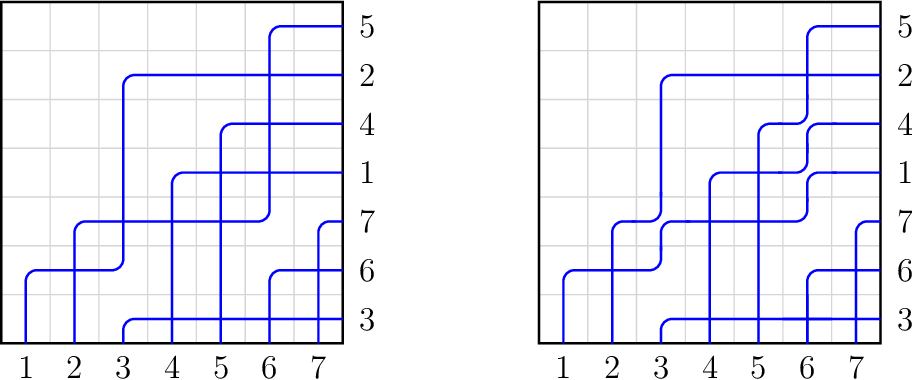
\includegraphics[scale=0.2]{bpd}
        \end{center}
    \end{definition}

    \begin{example}{}
        For $w=2143$, recall that
        \begin{equation*}
            z_{1,1},
            \det
            \begin{bmatrix}
                0 & z_{1,2} & z_{1,3} \\
                z_{2,1} & z_{2,2} & z_{2,3} \\
                z_{3,1} & z_{3,2} & z_{3,3} \\
            \end{bmatrix}
        \end{equation*}
        is a diagonal Grobner basis, and the initial ideal is
        \begin{equation*}
            \left< z_{1,1}, z_{1,2}z_{2,1}z_{3,3} \right> = \left< z_{1,1},z_{1,2} \right> \cap \left< z_{1,1},z_{2,1} \right> \cap \left< z_{1,1},z_{3,3} \right>.    
        \end{equation*}
        The associated bumpless pipe dreams are

        \begin{center}
            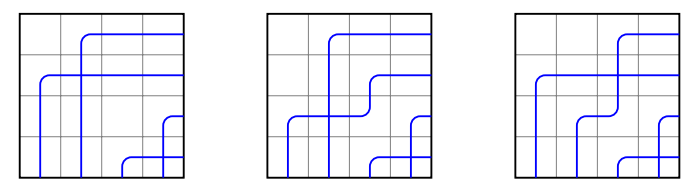
\includegraphics[scale=0.4]{bpd2143}
        \end{center}

        Observe that the prime ideals $\left< z_{1,1},z_{1,2} \right>, \left< z_{1,1},z_{2,1} \right>, \left< z_{1,1},z_{3,3} \right>$ biject with the pipe dreams by the coordinates of blank tiles.
    \end{example}
    
    \rruleline
    
    \begin{theorem}{Klein-Weigandt}
        For $w\in S_n$ and many diagonal orders, the radical of the initial ideal
        \begin{equation*}
            \sqrt{\initial_{\text{diag}}\left( I_w \right)} = \bigcap^{}_{P\in\text{bpd}\left( w \right)} \left< z_{i,j} : \text{$P$ has a blank tile in position $\left( i,j \right)$} \right> .
        \end{equation*}
        where $\text{bpd}\left( w \right)$ is the set of bumpless pipe dreams associated with $w$.

        Moreover, the degree of a component equals the number of bumpless pipe dreams with blank tiles in these positions.
    \end{theorem}
    
    \rruleline

    \clearpage
    
    \begin{example}{}
        Consider
        \begin{equation*}
            w = 321654\in S_6.
        \end{equation*}
        The corresponding bpd's are

        \begin{center}
            (picture)
        \end{center}

        Observe that the six northwest corners are blank in both diagrams, which means the corresponding variables have \textit{quadratic fuzz} in the scheme.
    \end{example}
    
    \rruleline
    
    \np We still do not know when $\initial_{\text{diag}}\left( I_w \right)$ is radical. Clearly permutations such that there are multiple bpd's with the same blank tile position are not radical. Even if different bpd's have blank tiles in different positisions, there could be some embedded components. The best guess so far is \textit{pattern avoidance}. From Example 3.33, it is clear that $321654$ is \textit{very bad}. The blank tiles appear in the same position in every bpd's.

    \subsection{Skew-symmetric Matries with Northwest Rank Conditions}

    Consider
    \begin{equation*}
        \mF = \left\lbrace X\in\F^{n\times n}: X^{T} = -X, \rank\left( X_{\left[ i \right],\left[ j \right]} \right) \leq r_{i,j} \right\rbrace
    \end{equation*}
    for some rank matrix $r\in\N^{n\times n}$. In case $\F = \Z_2$, we impose an extra condition that the diagonal entries of $X\in\mF$ are $0$.

    \np The irreducibles of $\mF$ are indexed by fixed-point free involutions $w\in S_n$. That is, $w^{2}\left( i \right) = i \neq w\left( i \right)$ for all $i\in\left[ n \right]$.

    \begin{theorem}{Marberg-Pawlowski}
        The defining determinants of $\mF$ do not generate a radical ideal.

        Instead, the radical ideal is generated by Pfaffians.\footnotemark[1] That is,
        \begin{equation*}
            \left< \sqrt{\det\left( A \right)}:A\in\mF \right> 
        \end{equation*}
        is a radical ideal. 

        A Grobner basis for the radical ideal is a set of Pfaffians to a \textit{particular antidiagonal order}. For this term order, the initial ideal is is squarefree and Cohen-Macaulay (the corresponding ASC is vertex-decomposable). The prime decomposition of the initial ideal is generated by \textit{pfp-involution pipe dreams}.
        
        \noindent
        \begin{minipage}{\textwidth}
            \footnotetext[1]{The square roots of $\det\left( A \right), A\in\mF$, which make sense since determinants of skew-symmetric matrices are perfect squares}
        \end{minipage}
    \end{theorem}
    
    \rruleline
    
    \np Here are some related questions.
    \begin{itemize}
        \item \textit{Skew symmetric matrices with southwest rank conditions?}
        \item \textit{Symmetric matrices? With southwest rank conditions?}
    \end{itemize} 
    Turns out symmetric matrices with southwest rank conditions are easier (but still hard) to deal with.
    
    \begin{theorem}{Fink-Rajchgot-Sullivant}
        For symmetric matrices with southwest rank conditions, defining equations form a diagoanal Grobner basis. The generated diagonal initial ideal is squarefree.
    \end{theorem}

    \rruleline
    
    \begin{theorem}{}
        Consider the setting of Theorem 3.46. The diagonal ideal is Cohen-Macaulay.
    \end{theorem}

    \begin{proof}[Proof Sketch]
        The diagonal initial is Stanley-Reisner ideal of a type C subword complex.
    \end{proof}

    \np The facets are given by type C pipe dreams.

    \begin{example}{Double Determinantal Variety}
        A \emph{double determinantal variety} is
        \begin{equation*}
            D_{m,n,r,s,t} = \left\lbrace \left( X_1,\ldots,X_r \right)\in \left( \F^{m\times n} \right)^r : \rank\left( \begin{bmatrix} X_1 & \cdots & X_r \end{bmatrix}\right) \leq s, \rank\left( \begin{bmatrix} X_1 \\ \vdots \\ X_r \end{bmatrix} \right)\leq t \right\rbrace.
        \end{equation*}
    \end{example}
    
    \rruleline
    
    \begin{theorem}{Fieldstell-Klein}
        The defining equations of $D_{m,n,r,s,t}$ form a Grobner basis under any diagonal or antidiagonal term order, which generates a prime ideal. The initial ideal is Stanlye-Reisner ideal of a vertex-decomposable ASC so both ideals are Cohen-Macaulay.
    \end{theorem}

    \rruleline
    
    \subsection{Edge Ideal of a Graph}
    
    Let $G$ be a simple graph on $\left[ n \right]$ and let
    \begin{equation*}
        I_G = \left< x_ix_j : ij\in E\left( G \right) \right>, 
    \end{equation*}
    called the \emph{edge ideal}.

    \begin{prop}{}
        $\dim\left( S /I_G \right) = \alpha\left( G \right)$, where $\alpha\left( G \right)$ is the size of the largest independent set in $G$ (i.e. set of vertices that are not adjacent).
    \end{prop}

    \rruleline
    
    \begin{theorem}{Hibi-Matsuda}
        For any $r,r'\geq 1$, there is a monomial ideal $I$ with
        \begin{equation*}
            \reg\left( S /I \right) = r
        \end{equation*}
        and
        \begin{equation*}
            \deg\left( K\left( S /I, t \right) \right) - \codim\left( S /I \right) = r'.
        \end{equation*}
    \end{theorem}

    \rruleline

    \begin{theorem}{Hibi-Matsuda-van Tvyl}
        For any $r,r'\geq 1$, there is a graph $G$ with
        \begin{equation*}
            \reg\left( S /I_G \right) = r
        \end{equation*}
        and
        \begin{equation*}
            \deg\left( K\left( S/ I_G, t \right) \right) - \codim\left( S /I_G \right) = r'.
        \end{equation*}
        However, if $\left| V\left( G \right) \right| = n$, then
        \begin{equation*}
            \dim\left( S /I_G  \right) +\deg\left( K\left( S /I,t \right) \right) - \codim\left( S /I_G \right) \leq n.
        \end{equation*}
    \end{theorem}

    \rruleline

    
    
    
    
    
    
    
    
    
    
    
    
    
    
    
    
    
    
    
    
    
    
    
    
    
    
    
    
    
    
    
    
    
    
    
    


\end{document}
